% Options for packages loaded elsewhere
\PassOptionsToPackage{unicode}{hyperref}
\PassOptionsToPackage{hyphens}{url}
%
\documentclass[
]{article}
\usepackage{amsmath,amssymb}
\usepackage{lmodern}
\usepackage{iftex}
\ifPDFTeX
  \usepackage[T1]{fontenc}
  \usepackage[utf8]{inputenc}
  \usepackage{textcomp} % provide euro and other symbols
\else % if luatex or xetex
  \usepackage{unicode-math}
  \defaultfontfeatures{Scale=MatchLowercase}
  \defaultfontfeatures[\rmfamily]{Ligatures=TeX,Scale=1}
\fi
% Use upquote if available, for straight quotes in verbatim environments
\IfFileExists{upquote.sty}{\usepackage{upquote}}{}
\IfFileExists{microtype.sty}{% use microtype if available
  \usepackage[]{microtype}
  \UseMicrotypeSet[protrusion]{basicmath} % disable protrusion for tt fonts
}{}
\makeatletter
\@ifundefined{KOMAClassName}{% if non-KOMA class
  \IfFileExists{parskip.sty}{%
    \usepackage{parskip}
  }{% else
    \setlength{\parindent}{0pt}
    \setlength{\parskip}{6pt plus 2pt minus 1pt}}
}{% if KOMA class
  \KOMAoptions{parskip=half}}
\makeatother
\usepackage{xcolor}
\usepackage[margin=1in]{geometry}
\usepackage{color}
\usepackage{fancyvrb}
\newcommand{\VerbBar}{|}
\newcommand{\VERB}{\Verb[commandchars=\\\{\}]}
\DefineVerbatimEnvironment{Highlighting}{Verbatim}{commandchars=\\\{\}}
% Add ',fontsize=\small' for more characters per line
\usepackage{framed}
\definecolor{shadecolor}{RGB}{248,248,248}
\newenvironment{Shaded}{\begin{snugshade}}{\end{snugshade}}
\newcommand{\AlertTok}[1]{\textcolor[rgb]{0.94,0.16,0.16}{#1}}
\newcommand{\AnnotationTok}[1]{\textcolor[rgb]{0.56,0.35,0.01}{\textbf{\textit{#1}}}}
\newcommand{\AttributeTok}[1]{\textcolor[rgb]{0.77,0.63,0.00}{#1}}
\newcommand{\BaseNTok}[1]{\textcolor[rgb]{0.00,0.00,0.81}{#1}}
\newcommand{\BuiltInTok}[1]{#1}
\newcommand{\CharTok}[1]{\textcolor[rgb]{0.31,0.60,0.02}{#1}}
\newcommand{\CommentTok}[1]{\textcolor[rgb]{0.56,0.35,0.01}{\textit{#1}}}
\newcommand{\CommentVarTok}[1]{\textcolor[rgb]{0.56,0.35,0.01}{\textbf{\textit{#1}}}}
\newcommand{\ConstantTok}[1]{\textcolor[rgb]{0.00,0.00,0.00}{#1}}
\newcommand{\ControlFlowTok}[1]{\textcolor[rgb]{0.13,0.29,0.53}{\textbf{#1}}}
\newcommand{\DataTypeTok}[1]{\textcolor[rgb]{0.13,0.29,0.53}{#1}}
\newcommand{\DecValTok}[1]{\textcolor[rgb]{0.00,0.00,0.81}{#1}}
\newcommand{\DocumentationTok}[1]{\textcolor[rgb]{0.56,0.35,0.01}{\textbf{\textit{#1}}}}
\newcommand{\ErrorTok}[1]{\textcolor[rgb]{0.64,0.00,0.00}{\textbf{#1}}}
\newcommand{\ExtensionTok}[1]{#1}
\newcommand{\FloatTok}[1]{\textcolor[rgb]{0.00,0.00,0.81}{#1}}
\newcommand{\FunctionTok}[1]{\textcolor[rgb]{0.00,0.00,0.00}{#1}}
\newcommand{\ImportTok}[1]{#1}
\newcommand{\InformationTok}[1]{\textcolor[rgb]{0.56,0.35,0.01}{\textbf{\textit{#1}}}}
\newcommand{\KeywordTok}[1]{\textcolor[rgb]{0.13,0.29,0.53}{\textbf{#1}}}
\newcommand{\NormalTok}[1]{#1}
\newcommand{\OperatorTok}[1]{\textcolor[rgb]{0.81,0.36,0.00}{\textbf{#1}}}
\newcommand{\OtherTok}[1]{\textcolor[rgb]{0.56,0.35,0.01}{#1}}
\newcommand{\PreprocessorTok}[1]{\textcolor[rgb]{0.56,0.35,0.01}{\textit{#1}}}
\newcommand{\RegionMarkerTok}[1]{#1}
\newcommand{\SpecialCharTok}[1]{\textcolor[rgb]{0.00,0.00,0.00}{#1}}
\newcommand{\SpecialStringTok}[1]{\textcolor[rgb]{0.31,0.60,0.02}{#1}}
\newcommand{\StringTok}[1]{\textcolor[rgb]{0.31,0.60,0.02}{#1}}
\newcommand{\VariableTok}[1]{\textcolor[rgb]{0.00,0.00,0.00}{#1}}
\newcommand{\VerbatimStringTok}[1]{\textcolor[rgb]{0.31,0.60,0.02}{#1}}
\newcommand{\WarningTok}[1]{\textcolor[rgb]{0.56,0.35,0.01}{\textbf{\textit{#1}}}}
\usepackage{graphicx}
\makeatletter
\def\maxwidth{\ifdim\Gin@nat@width>\linewidth\linewidth\else\Gin@nat@width\fi}
\def\maxheight{\ifdim\Gin@nat@height>\textheight\textheight\else\Gin@nat@height\fi}
\makeatother
% Scale images if necessary, so that they will not overflow the page
% margins by default, and it is still possible to overwrite the defaults
% using explicit options in \includegraphics[width, height, ...]{}
\setkeys{Gin}{width=\maxwidth,height=\maxheight,keepaspectratio}
% Set default figure placement to htbp
\makeatletter
\def\fps@figure{htbp}
\makeatother
\setlength{\emergencystretch}{3em} % prevent overfull lines
\providecommand{\tightlist}{%
  \setlength{\itemsep}{0pt}\setlength{\parskip}{0pt}}
\setcounter{secnumdepth}{5}
\ifLuaTeX
  \usepackage{selnolig}  % disable illegal ligatures
\fi
\IfFileExists{bookmark.sty}{\usepackage{bookmark}}{\usepackage{hyperref}}
\IfFileExists{xurl.sty}{\usepackage{xurl}}{} % add URL line breaks if available
\urlstyle{same} % disable monospaced font for URLs
\hypersetup{
  pdftitle={HUDM6122 Homework\_02},
  pdfauthor={Chenguang Pan},
  hidelinks,
  pdfcreator={LaTeX via pandoc}}

\title{HUDM6122 Homework\_02}
\author{Chenguang Pan}
\date{2023-02-06}

\begin{document}
\maketitle

\hypertarget{ex.-2.1}{%
\subsection{Ex. 2.1}\label{ex.-2.1}}

\emph{Use the bivariate boxplot on the scatterplot of each pair of
variables in the air pollution data to identify any outliers. Calculate
the correlation between each pair of variables using all the data and
the data with any identified outliers removed. Comment on the results.}

\textbf{MY SOLUTION:}

Several techniques worth to be noted: - use a for-loop within a for-loop
to map all pairs - use \texttt{text()} to give each point a name. - the
bivariate boxplot function \texttt{bvbox} is inclueded in the package
\texttt{MVA}

\begin{Shaded}
\begin{Highlighting}[]
\SpecialCharTok{\textgreater{}} \CommentTok{\# import the data}
\ErrorTok{\textgreater{}} \FunctionTok{library}\NormalTok{(HSAUR2)}
\SpecialCharTok{\textgreater{}} \FunctionTok{library}\NormalTok{(MVA)}
\SpecialCharTok{\textgreater{}} \FunctionTok{attach}\NormalTok{(USairpollution)}
\SpecialCharTok{\textgreater{}} \FunctionTok{head}\NormalTok{(USairpollution)}
\NormalTok{            SO2 temp manu popul wind precip predays}
\NormalTok{Albany       }\DecValTok{46} \FloatTok{47.6}   \DecValTok{44}   \DecValTok{116}  \FloatTok{8.8}  \FloatTok{33.36}     \DecValTok{135}
\NormalTok{Albuquerque  }\DecValTok{11} \FloatTok{56.8}   \DecValTok{46}   \DecValTok{244}  \FloatTok{8.9}   \FloatTok{7.77}      \DecValTok{58}
\NormalTok{Atlanta      }\DecValTok{24} \FloatTok{61.5}  \DecValTok{368}   \DecValTok{497}  \FloatTok{9.1}  \FloatTok{48.34}     \DecValTok{115}
\NormalTok{Baltimore    }\DecValTok{47} \FloatTok{55.0}  \DecValTok{625}   \DecValTok{905}  \FloatTok{9.6}  \FloatTok{41.31}     \DecValTok{111}
\NormalTok{Buffalo      }\DecValTok{11} \FloatTok{47.1}  \DecValTok{391}   \DecValTok{463} \FloatTok{12.4}  \FloatTok{36.11}     \DecValTok{166}
\NormalTok{Charleston   }\DecValTok{31} \FloatTok{55.2}   \DecValTok{35}    \DecValTok{71}  \FloatTok{6.5}  \FloatTok{40.75}     \DecValTok{148}
\SpecialCharTok{\textgreater{}} \FunctionTok{dim}\NormalTok{(USairpollution)}
\NormalTok{[}\DecValTok{1}\NormalTok{] }\DecValTok{41}  \DecValTok{7}
\SpecialCharTok{\textgreater{}} \CommentTok{\# draw the bivariate boxplot of each pair of variables with a for{-}loop}
\ErrorTok{\textgreater{}} \ControlFlowTok{for}\NormalTok{ (i }\ControlFlowTok{in} \DecValTok{1}\SpecialCharTok{:}\DecValTok{7}\NormalTok{) \{}
\SpecialCharTok{+}   \ControlFlowTok{for}\NormalTok{ (j }\ControlFlowTok{in}\NormalTok{ i}\SpecialCharTok{:}\DecValTok{7}\NormalTok{) \{}
\SpecialCharTok{+}     \ControlFlowTok{if}\NormalTok{ (i }\SpecialCharTok{!=}\NormalTok{ j) \{}
\SpecialCharTok{+}\NormalTok{       var\_pair }\OtherTok{\textless{}{-}}\NormalTok{ USairpollution[, }\FunctionTok{c}\NormalTok{(i, j)]}
\SpecialCharTok{+}       \FunctionTok{bvbox}\NormalTok{(var\_pair, }
\SpecialCharTok{+}             \AttributeTok{xlab =} \FunctionTok{names}\NormalTok{(USairpollution)[i],}
\SpecialCharTok{+}             \AttributeTok{ylab =} \FunctionTok{names}\NormalTok{(USairpollution)[j])}
\SpecialCharTok{+}       \FunctionTok{text}\NormalTok{(USairpollution[,i],USairpollution[,j],}
\SpecialCharTok{+}           \FunctionTok{row.names}\NormalTok{(USairpollution), }\CommentTok{\# to add the point name}
\SpecialCharTok{+}           \AttributeTok{pos=}\DecValTok{2}\NormalTok{,}\AttributeTok{col =} \StringTok{"blue"}\NormalTok{)}
\SpecialCharTok{+}\NormalTok{     \} }
\SpecialCharTok{+}\NormalTok{   \}}
\SpecialCharTok{+}\NormalTok{ \}}
\end{Highlighting}
\end{Shaded}

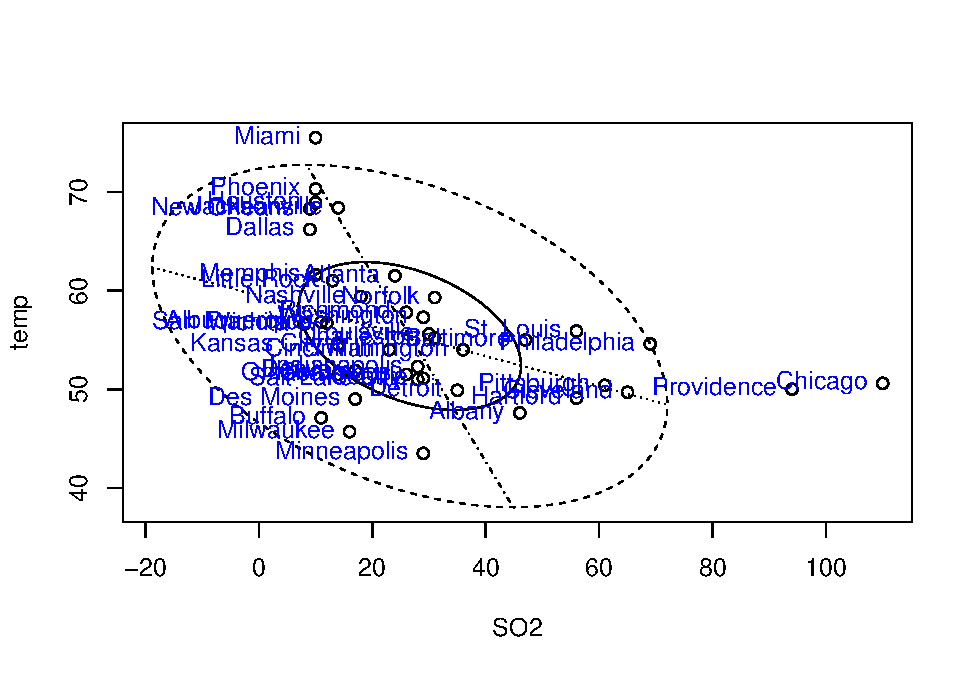
\includegraphics[width=0.33\linewidth,height=0.25\textheight]{HUDM6122-Homework_02-Chenguang-Pan_files/figure-latex/unnamed-chunk-1-1}
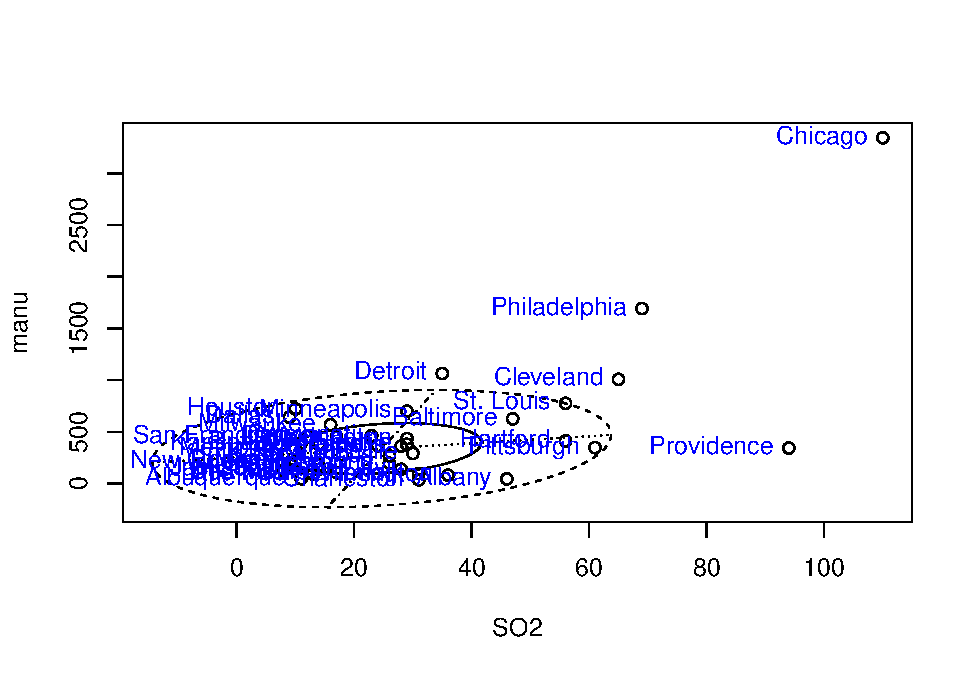
\includegraphics[width=0.33\linewidth,height=0.25\textheight]{HUDM6122-Homework_02-Chenguang-Pan_files/figure-latex/unnamed-chunk-1-2}
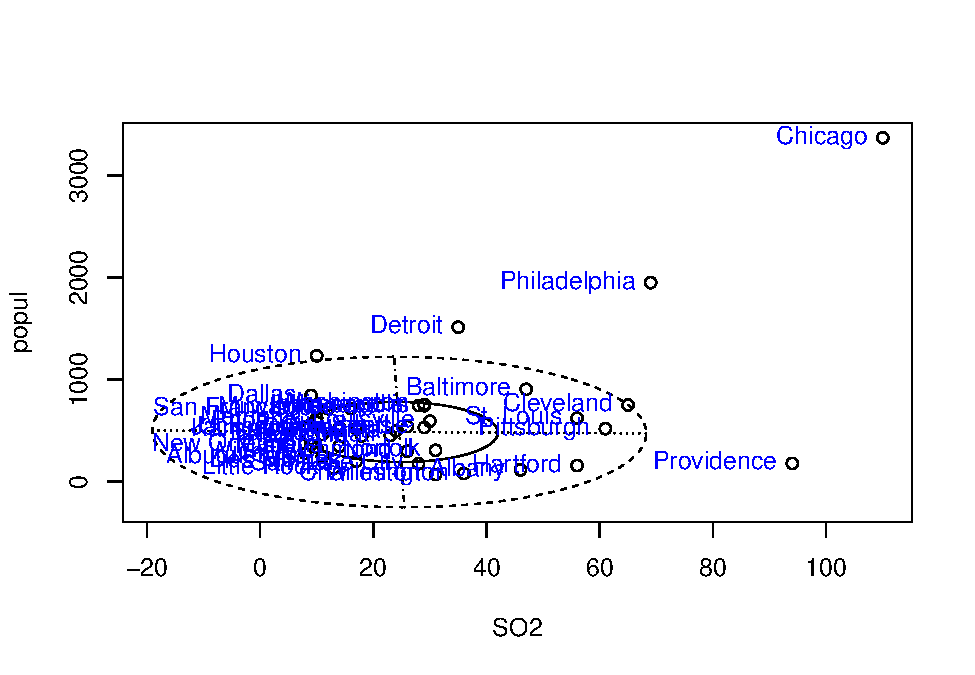
\includegraphics[width=0.33\linewidth,height=0.25\textheight]{HUDM6122-Homework_02-Chenguang-Pan_files/figure-latex/unnamed-chunk-1-3}
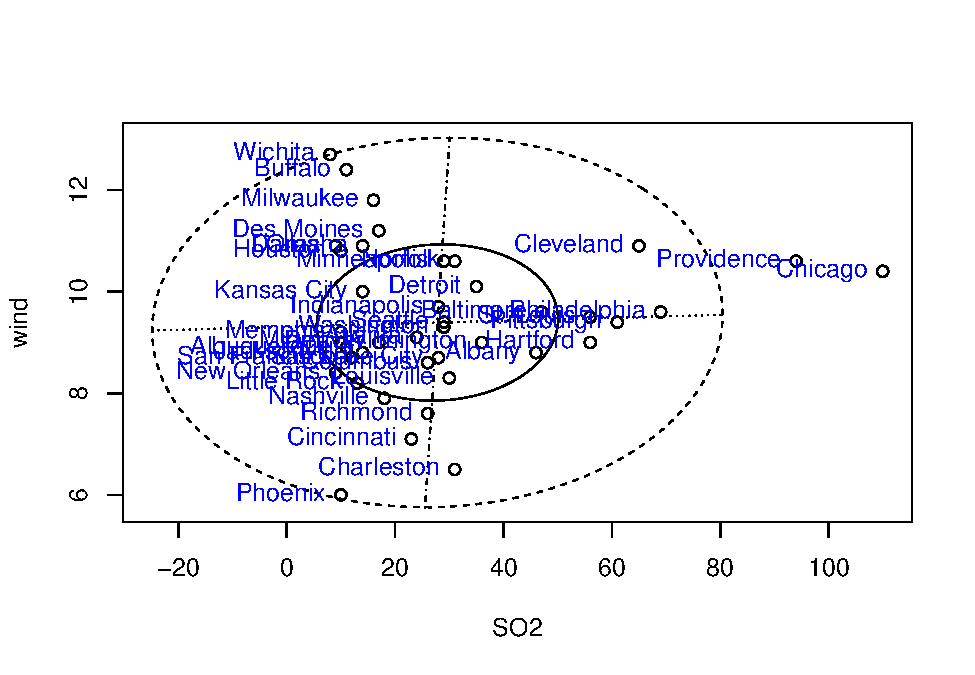
\includegraphics[width=0.33\linewidth,height=0.25\textheight]{HUDM6122-Homework_02-Chenguang-Pan_files/figure-latex/unnamed-chunk-1-4}
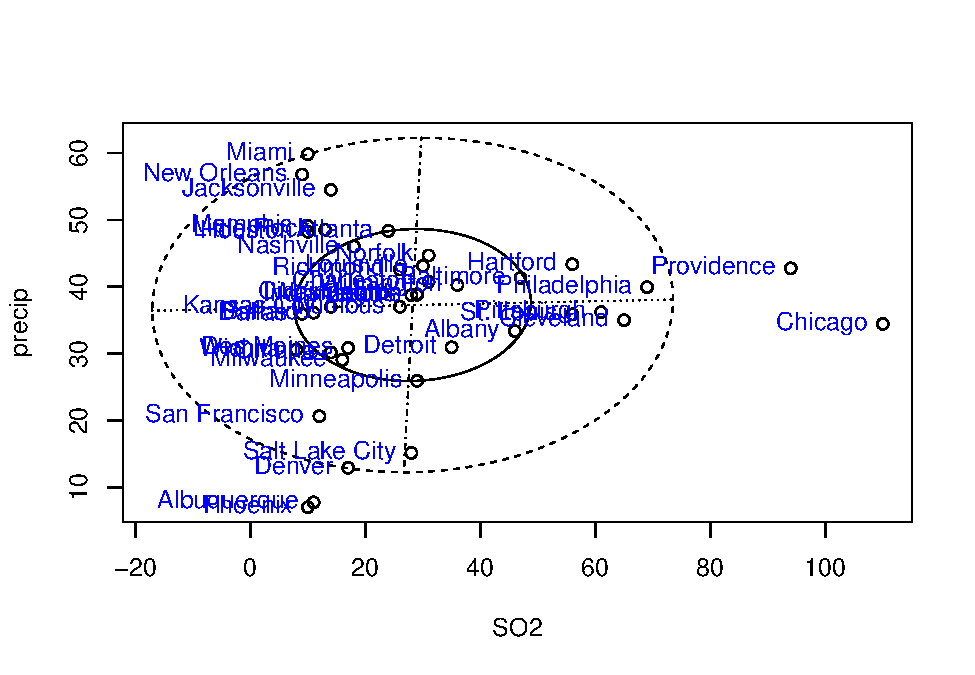
\includegraphics[width=0.33\linewidth,height=0.25\textheight]{HUDM6122-Homework_02-Chenguang-Pan_files/figure-latex/unnamed-chunk-1-5}
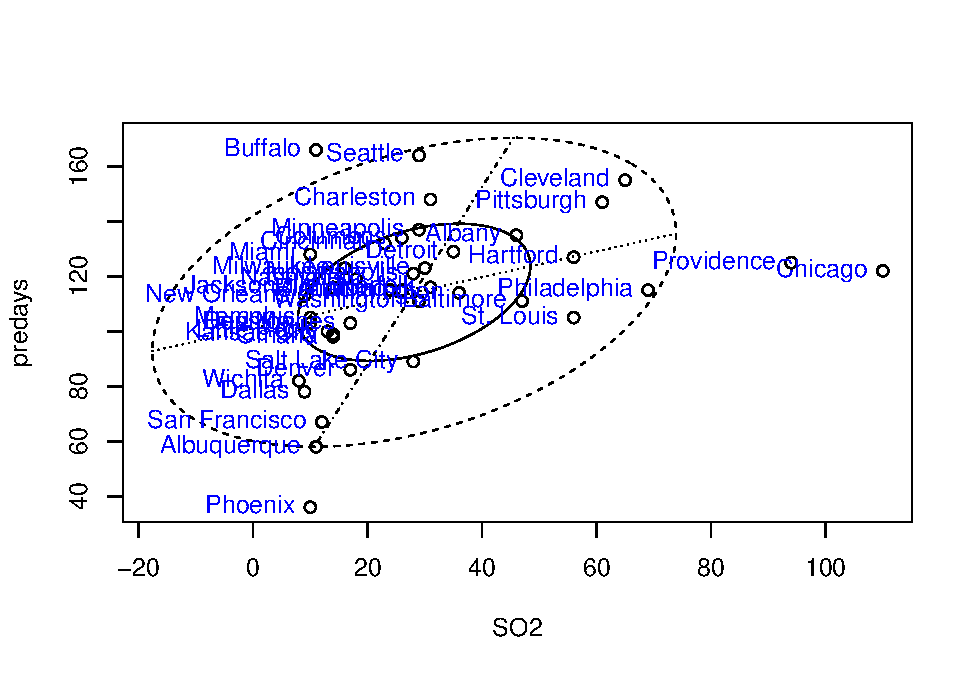
\includegraphics[width=0.33\linewidth,height=0.25\textheight]{HUDM6122-Homework_02-Chenguang-Pan_files/figure-latex/unnamed-chunk-1-6}
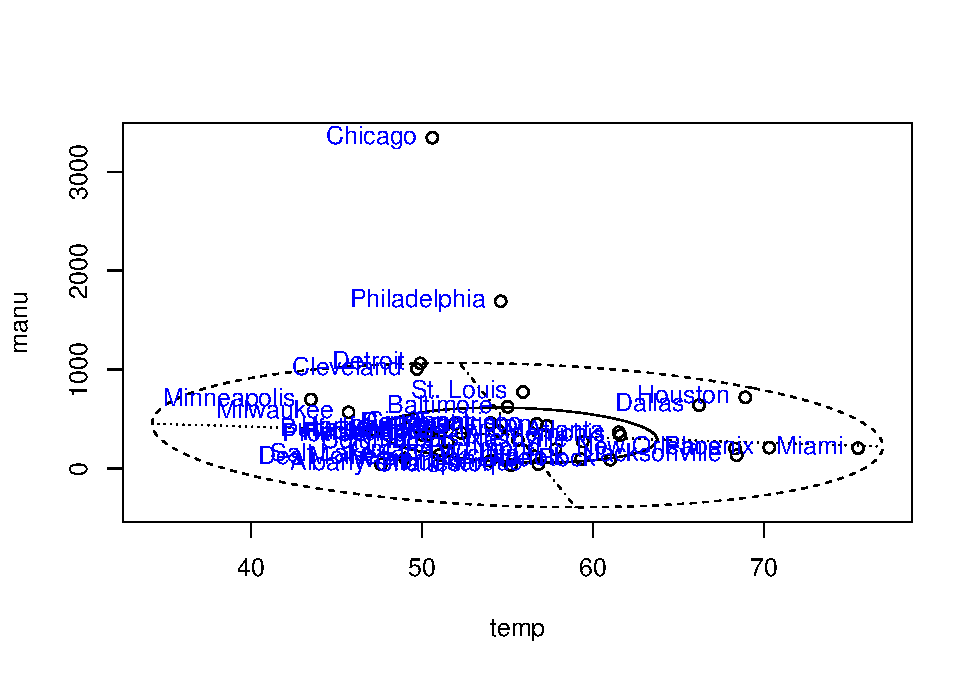
\includegraphics[width=0.33\linewidth,height=0.25\textheight]{HUDM6122-Homework_02-Chenguang-Pan_files/figure-latex/unnamed-chunk-1-7}
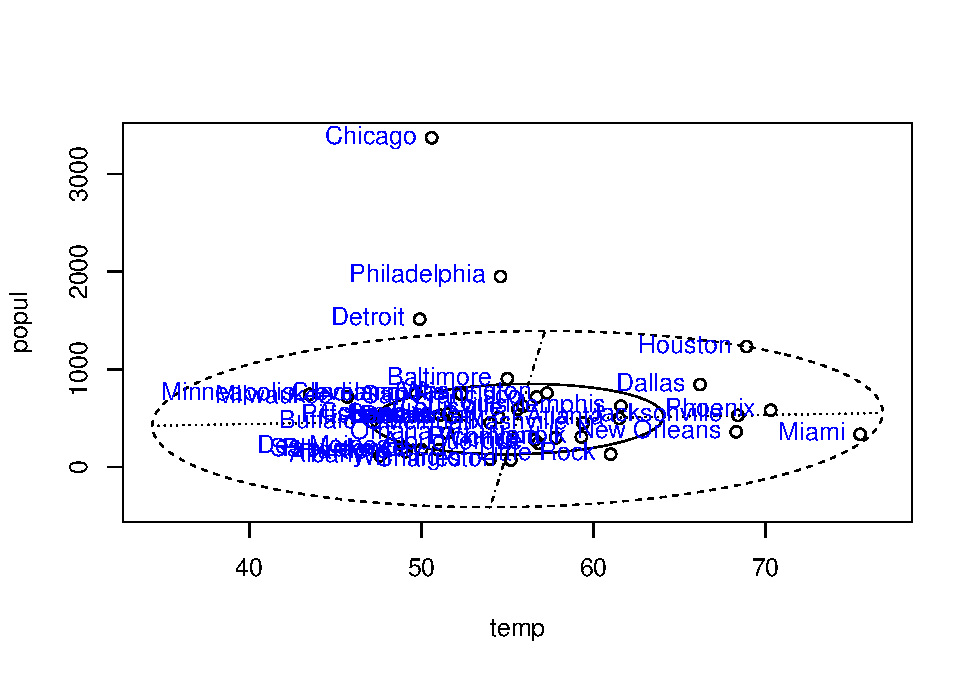
\includegraphics[width=0.33\linewidth,height=0.25\textheight]{HUDM6122-Homework_02-Chenguang-Pan_files/figure-latex/unnamed-chunk-1-8}
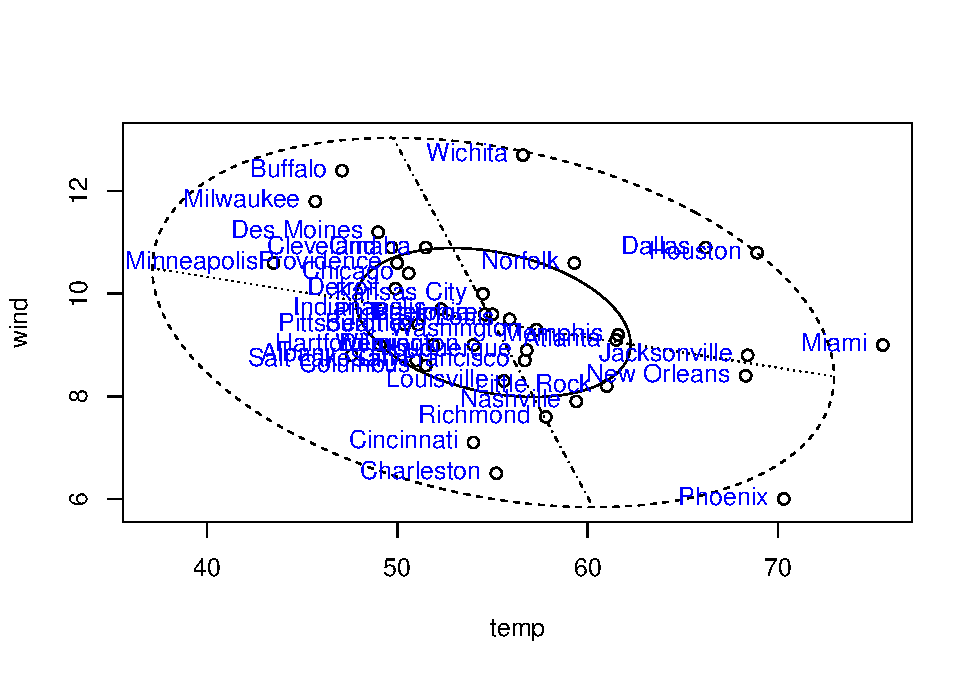
\includegraphics[width=0.33\linewidth,height=0.25\textheight]{HUDM6122-Homework_02-Chenguang-Pan_files/figure-latex/unnamed-chunk-1-9}
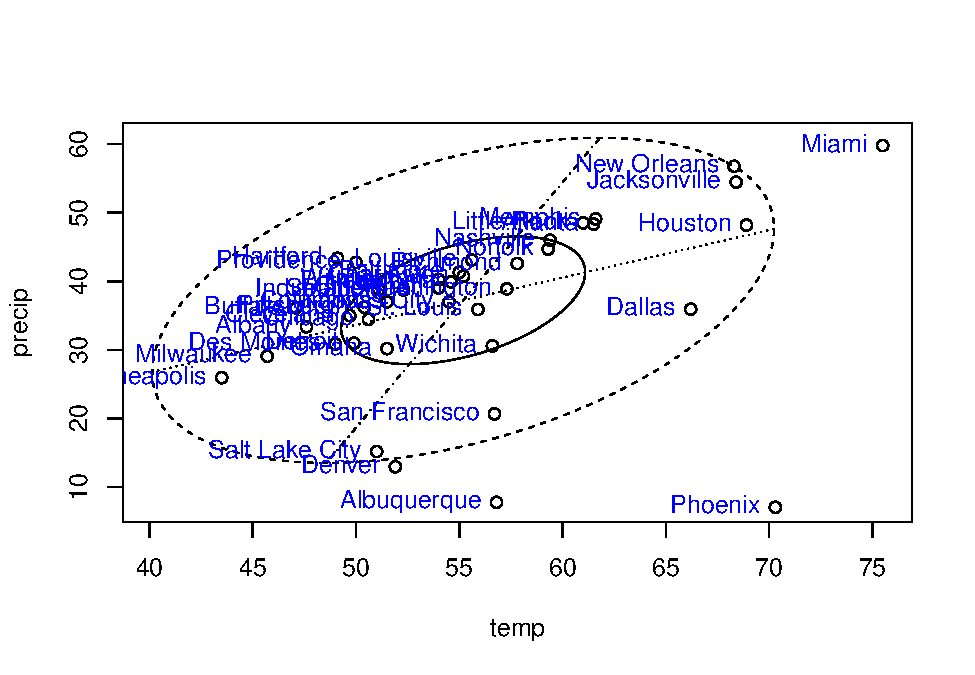
\includegraphics[width=0.33\linewidth,height=0.25\textheight]{HUDM6122-Homework_02-Chenguang-Pan_files/figure-latex/unnamed-chunk-1-10}
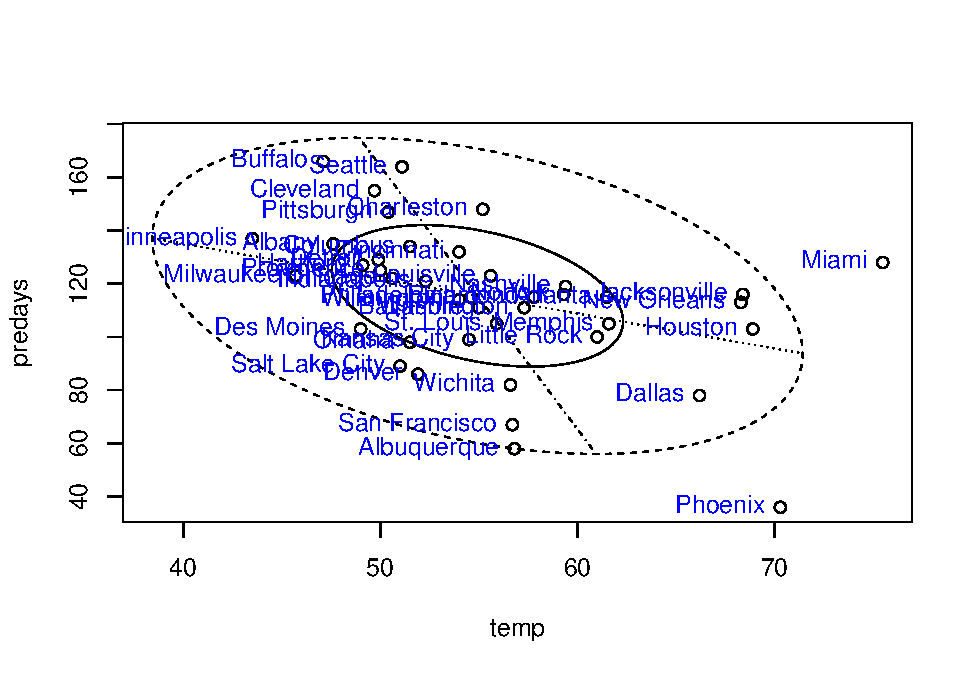
\includegraphics[width=0.33\linewidth,height=0.25\textheight]{HUDM6122-Homework_02-Chenguang-Pan_files/figure-latex/unnamed-chunk-1-11}
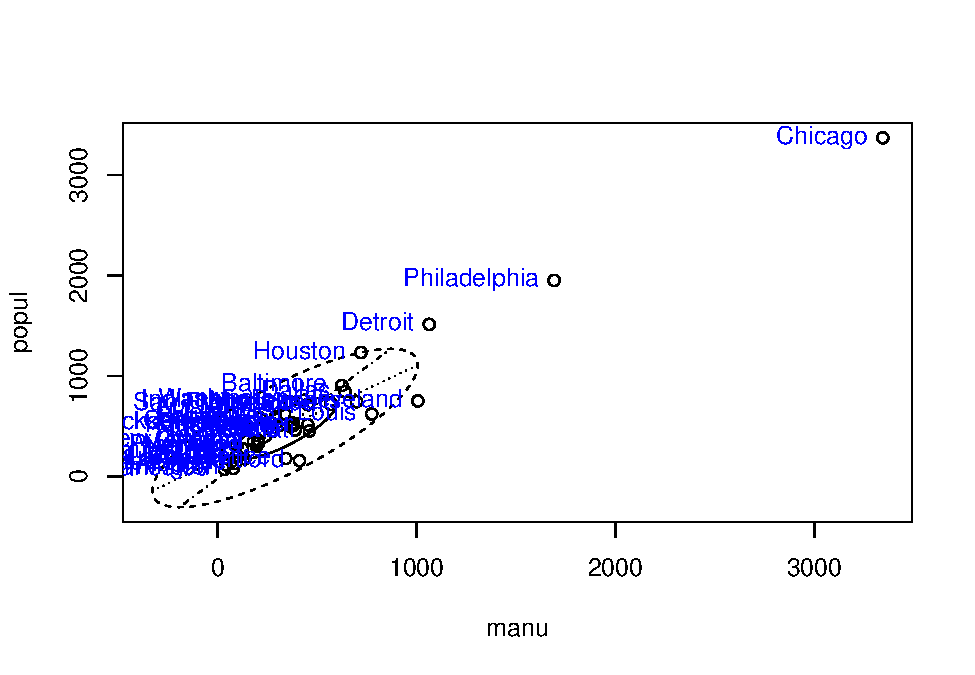
\includegraphics[width=0.33\linewidth,height=0.25\textheight]{HUDM6122-Homework_02-Chenguang-Pan_files/figure-latex/unnamed-chunk-1-12}
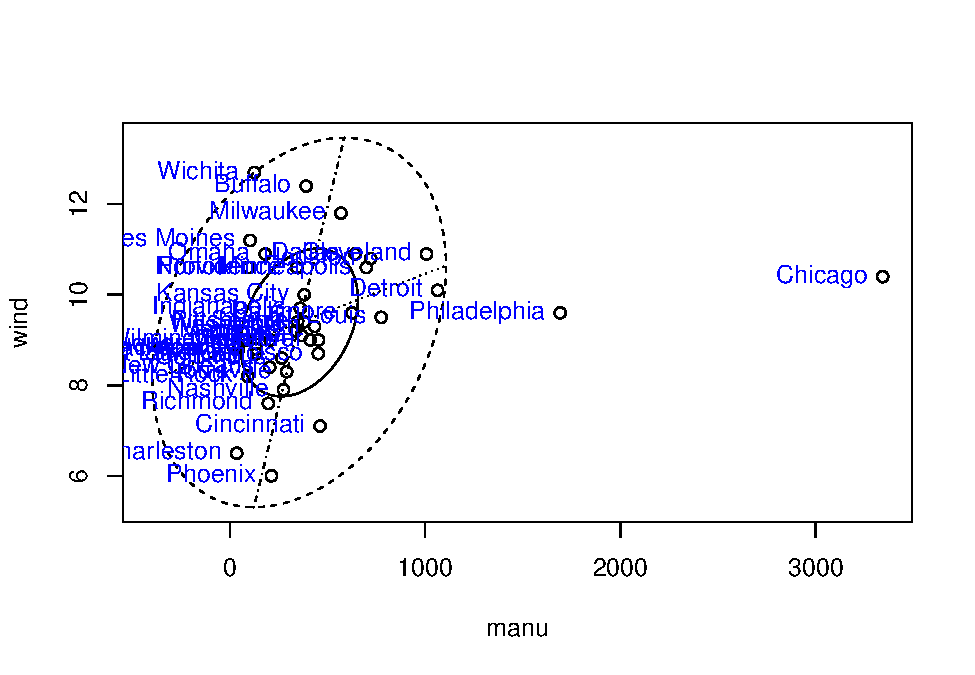
\includegraphics[width=0.33\linewidth,height=0.25\textheight]{HUDM6122-Homework_02-Chenguang-Pan_files/figure-latex/unnamed-chunk-1-13}
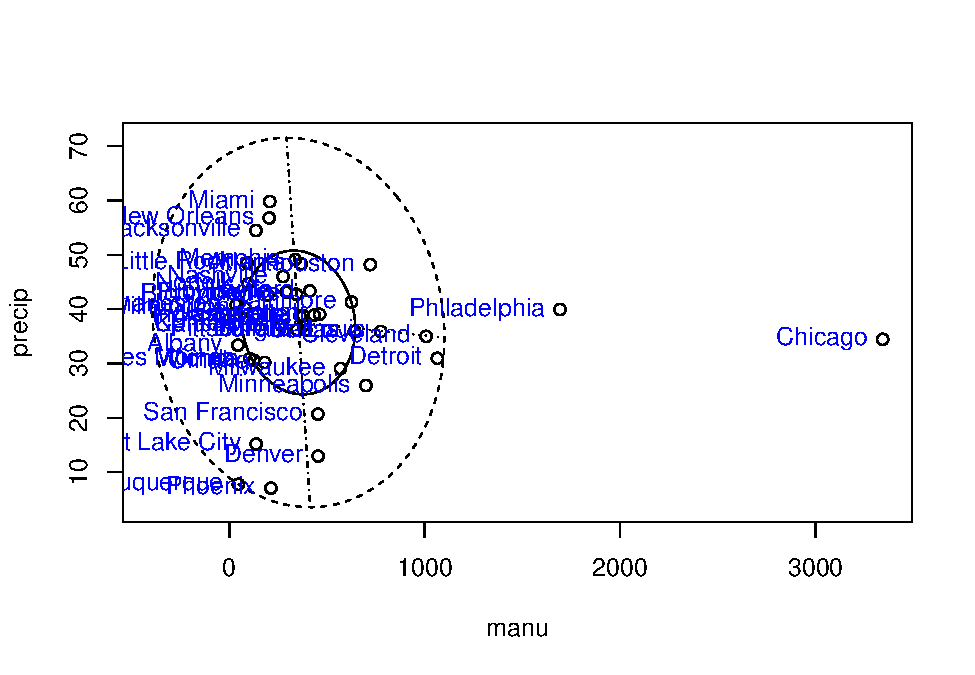
\includegraphics[width=0.33\linewidth,height=0.25\textheight]{HUDM6122-Homework_02-Chenguang-Pan_files/figure-latex/unnamed-chunk-1-14}
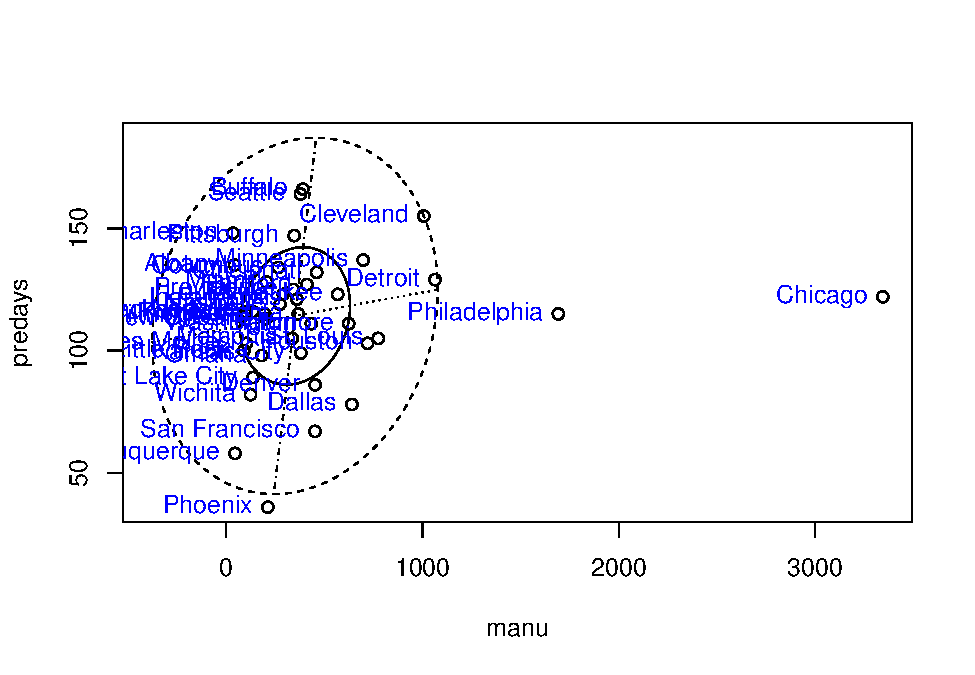
\includegraphics[width=0.33\linewidth,height=0.25\textheight]{HUDM6122-Homework_02-Chenguang-Pan_files/figure-latex/unnamed-chunk-1-15}
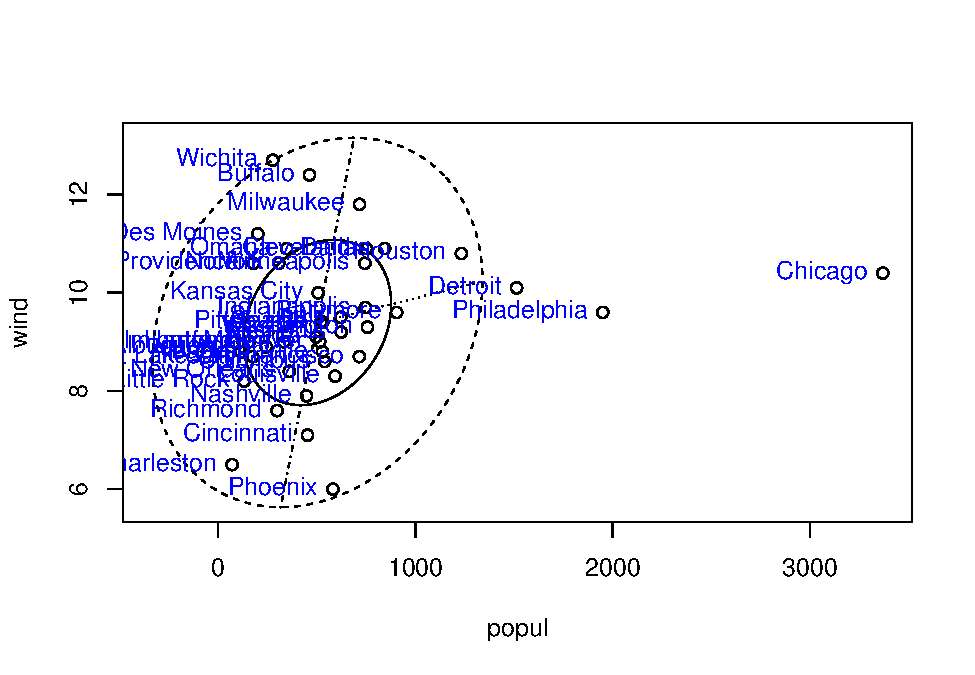
\includegraphics[width=0.33\linewidth,height=0.25\textheight]{HUDM6122-Homework_02-Chenguang-Pan_files/figure-latex/unnamed-chunk-1-16}
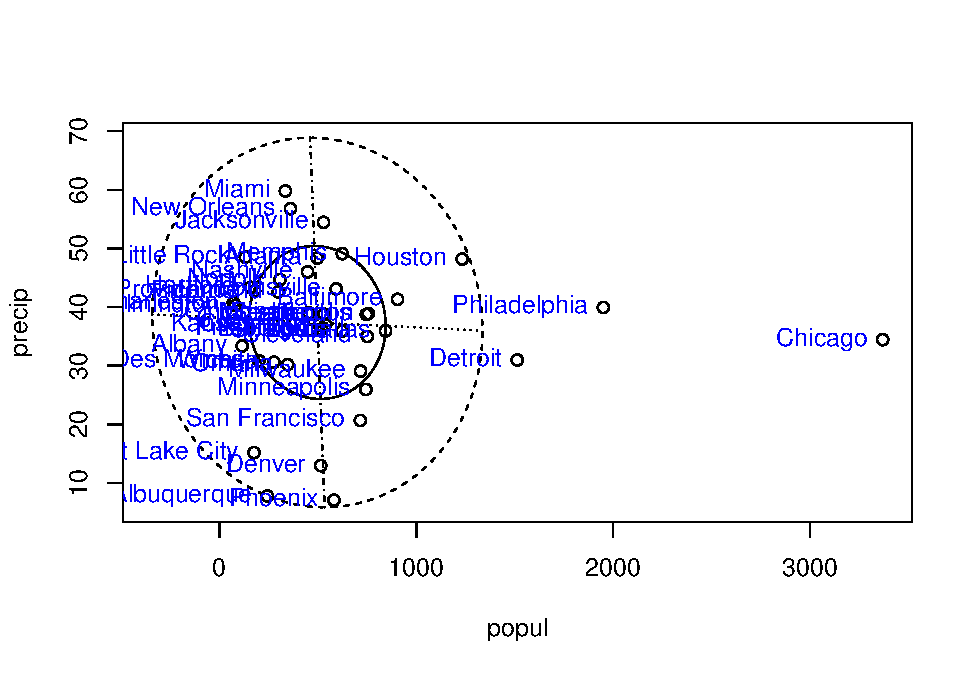
\includegraphics[width=0.33\linewidth,height=0.25\textheight]{HUDM6122-Homework_02-Chenguang-Pan_files/figure-latex/unnamed-chunk-1-17}
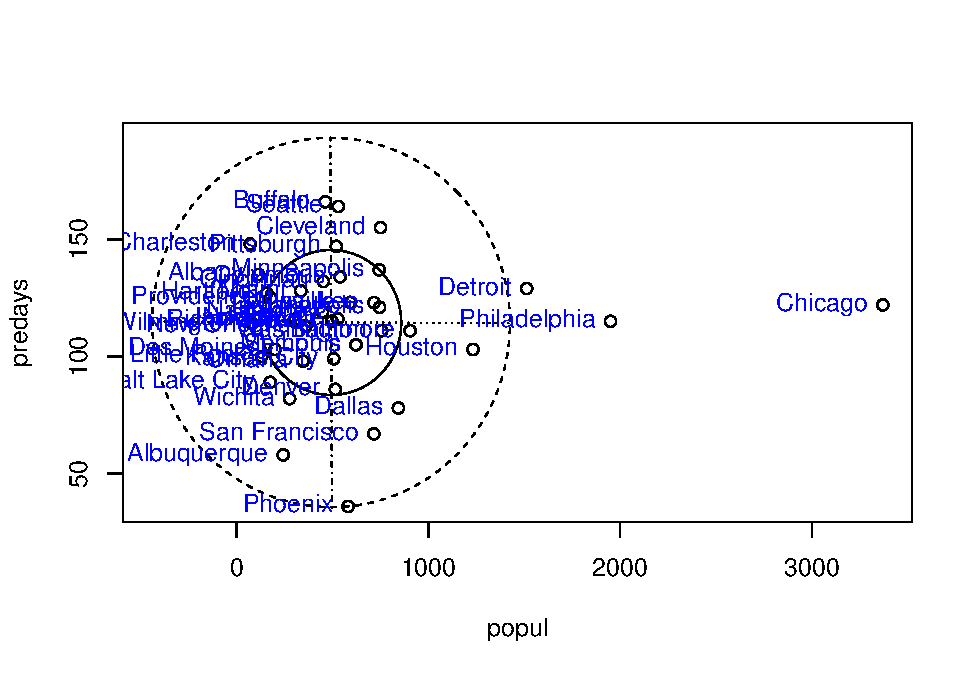
\includegraphics[width=0.33\linewidth,height=0.25\textheight]{HUDM6122-Homework_02-Chenguang-Pan_files/figure-latex/unnamed-chunk-1-18}
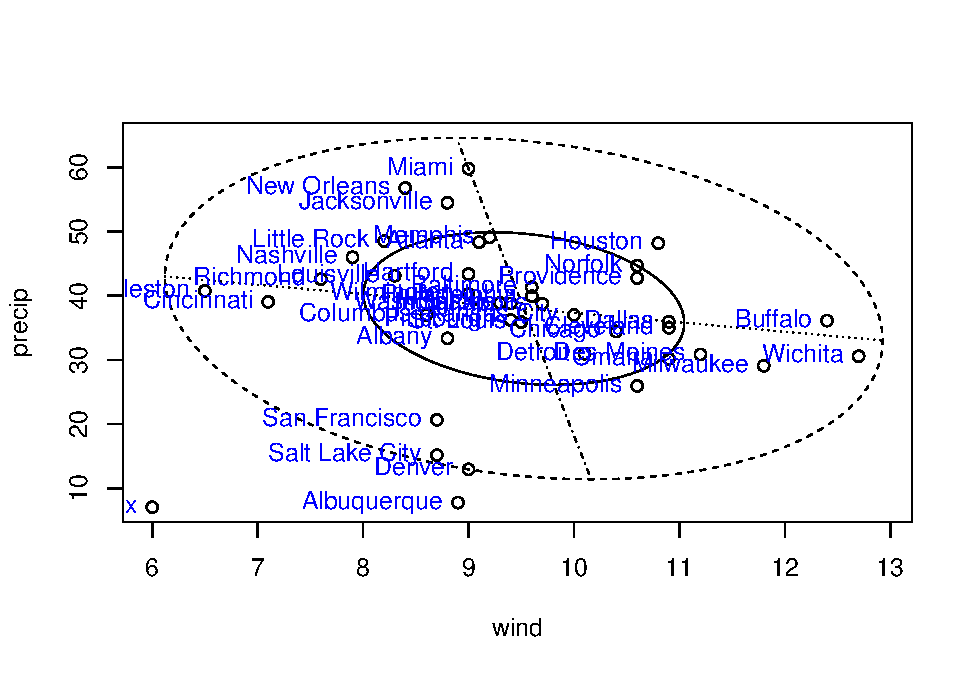
\includegraphics[width=0.33\linewidth,height=0.25\textheight]{HUDM6122-Homework_02-Chenguang-Pan_files/figure-latex/unnamed-chunk-1-19}
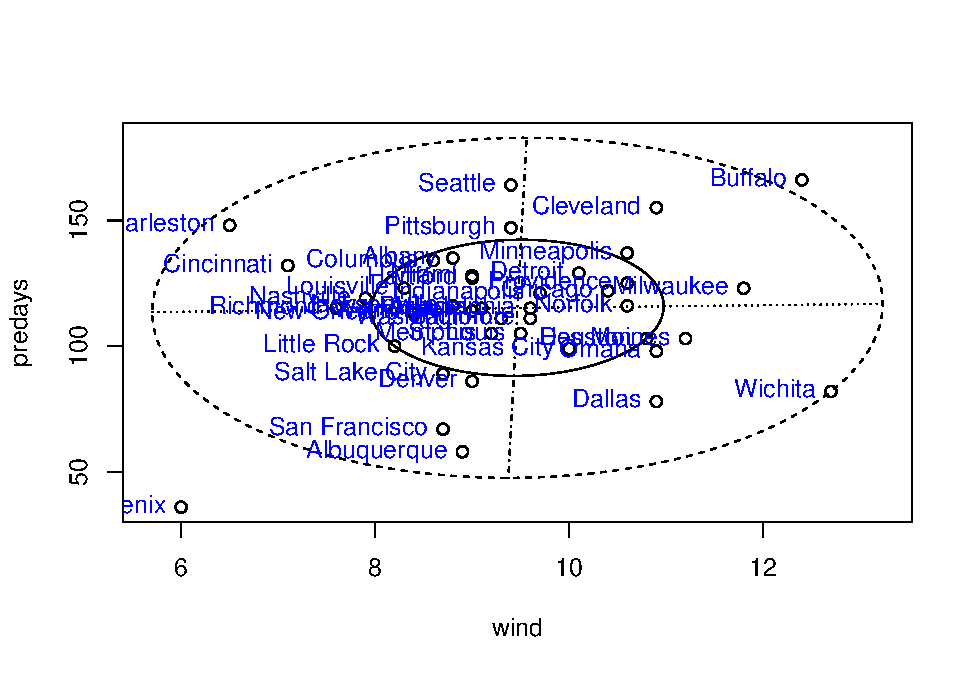
\includegraphics[width=0.33\linewidth,height=0.25\textheight]{HUDM6122-Homework_02-Chenguang-Pan_files/figure-latex/unnamed-chunk-1-20}
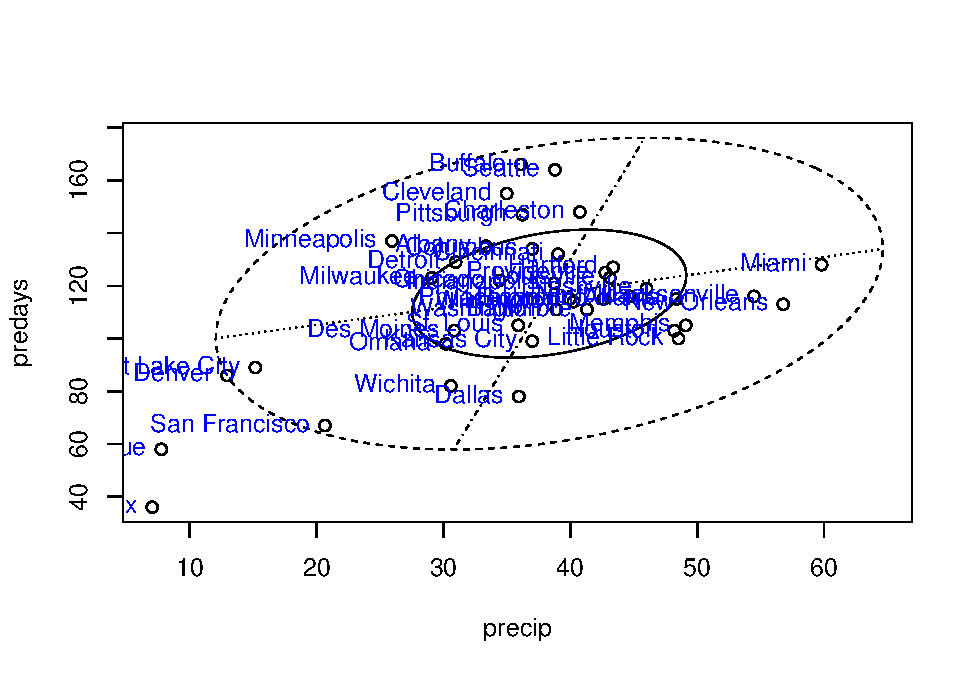
\includegraphics[width=0.33\linewidth,height=0.25\textheight]{HUDM6122-Homework_02-Chenguang-Pan_files/figure-latex/unnamed-chunk-1-21}
From the graphs, we can easily find that the outliers among the
observations are ``Chicago'', ``Detroit'',
``Cleveland'',``Philadelphia'', ``Miami'', ``Phoenix'',``Albuquerque'',
``Providence''. I run the correlation matrix on all observations first.

\begin{Shaded}
\begin{Highlighting}[]
\SpecialCharTok{\textgreater{}} \CommentTok{\# create the correaltion matrix on all observations}
\ErrorTok{\textgreater{}} \FunctionTok{round}\NormalTok{(}\FunctionTok{cor}\NormalTok{(USairpollution),}\DecValTok{2}\NormalTok{)}
\NormalTok{          SO2  temp  manu popul  wind precip predays}
\NormalTok{SO2      }\FloatTok{1.00} \SpecialCharTok{{-}}\FloatTok{0.43}  \FloatTok{0.64}  \FloatTok{0.49}  \FloatTok{0.09}   \FloatTok{0.05}    \FloatTok{0.37}
\NormalTok{temp    }\SpecialCharTok{{-}}\FloatTok{0.43}  \FloatTok{1.00} \SpecialCharTok{{-}}\FloatTok{0.19} \SpecialCharTok{{-}}\FloatTok{0.06} \SpecialCharTok{{-}}\FloatTok{0.35}   \FloatTok{0.39}   \SpecialCharTok{{-}}\FloatTok{0.43}
\NormalTok{manu     }\FloatTok{0.64} \SpecialCharTok{{-}}\FloatTok{0.19}  \FloatTok{1.00}  \FloatTok{0.96}  \FloatTok{0.24}  \SpecialCharTok{{-}}\FloatTok{0.03}    \FloatTok{0.13}
\NormalTok{popul    }\FloatTok{0.49} \SpecialCharTok{{-}}\FloatTok{0.06}  \FloatTok{0.96}  \FloatTok{1.00}  \FloatTok{0.21}  \SpecialCharTok{{-}}\FloatTok{0.03}    \FloatTok{0.04}
\NormalTok{wind     }\FloatTok{0.09} \SpecialCharTok{{-}}\FloatTok{0.35}  \FloatTok{0.24}  \FloatTok{0.21}  \FloatTok{1.00}  \SpecialCharTok{{-}}\FloatTok{0.01}    \FloatTok{0.16}
\NormalTok{precip   }\FloatTok{0.05}  \FloatTok{0.39} \SpecialCharTok{{-}}\FloatTok{0.03} \SpecialCharTok{{-}}\FloatTok{0.03} \SpecialCharTok{{-}}\FloatTok{0.01}   \FloatTok{1.00}    \FloatTok{0.50}
\NormalTok{predays  }\FloatTok{0.37} \SpecialCharTok{{-}}\FloatTok{0.43}  \FloatTok{0.13}  \FloatTok{0.04}  \FloatTok{0.16}   \FloatTok{0.50}    \FloatTok{1.00}
\SpecialCharTok{\textgreater{}} \CommentTok{\# remove all identified outliers}
\ErrorTok{\textgreater{}}\NormalTok{ drop\_city }\OtherTok{\textless{}{-}} \FunctionTok{match}\NormalTok{(}\FunctionTok{c}\NormalTok{(}\StringTok{"Chicago"}\NormalTok{, }\StringTok{"Detroit"}\NormalTok{,}\StringTok{"Cleveland"}\NormalTok{,}
\SpecialCharTok{+}                      \StringTok{"Philadelphia"}\NormalTok{, }\StringTok{"Miami"}\NormalTok{,}\StringTok{"Phoenix"}\NormalTok{,}
\SpecialCharTok{+}                      \StringTok{"Albuquerque"}\NormalTok{, }\StringTok{"Providence"}\NormalTok{), }\FunctionTok{rownames}\NormalTok{(USairpollution))}
\SpecialCharTok{\textgreater{}} 
\ErrorTok{\textgreater{}} \FunctionTok{round}\NormalTok{(}\FunctionTok{cor}\NormalTok{(USairpollution[}\SpecialCharTok{{-}}\NormalTok{drop\_city,]),}\DecValTok{2}\NormalTok{)}
\NormalTok{          SO2  temp  manu popul  wind precip predays}
\NormalTok{SO2      }\FloatTok{1.00} \SpecialCharTok{{-}}\FloatTok{0.40}  \FloatTok{0.10} \SpecialCharTok{{-}}\FloatTok{0.16} \SpecialCharTok{{-}}\FloatTok{0.26}  \SpecialCharTok{{-}}\FloatTok{0.03}    \FloatTok{0.39}
\NormalTok{temp    }\SpecialCharTok{{-}}\FloatTok{0.40}  \FloatTok{1.00} \SpecialCharTok{{-}}\FloatTok{0.02}  \FloatTok{0.25} \SpecialCharTok{{-}}\FloatTok{0.21}   \FloatTok{0.64}   \SpecialCharTok{{-}}\FloatTok{0.41}
\NormalTok{manu     }\FloatTok{0.10} \SpecialCharTok{{-}}\FloatTok{0.02}  \FloatTok{1.00}  \FloatTok{0.82}  \FloatTok{0.26}  \SpecialCharTok{{-}}\FloatTok{0.15}   \SpecialCharTok{{-}}\FloatTok{0.06}
\NormalTok{popul   }\SpecialCharTok{{-}}\FloatTok{0.16}  \FloatTok{0.25}  \FloatTok{0.82}  \FloatTok{1.00}  \FloatTok{0.29}   \FloatTok{0.03}   \SpecialCharTok{{-}}\FloatTok{0.13}
\NormalTok{wind    }\SpecialCharTok{{-}}\FloatTok{0.26} \SpecialCharTok{{-}}\FloatTok{0.21}  \FloatTok{0.26}  \FloatTok{0.29}  \FloatTok{1.00}  \SpecialCharTok{{-}}\FloatTok{0.26}   \SpecialCharTok{{-}}\FloatTok{0.13}
\NormalTok{precip  }\SpecialCharTok{{-}}\FloatTok{0.03}  \FloatTok{0.64} \SpecialCharTok{{-}}\FloatTok{0.15}  \FloatTok{0.03} \SpecialCharTok{{-}}\FloatTok{0.26}   \FloatTok{1.00}    \FloatTok{0.28}
\NormalTok{predays  }\FloatTok{0.39} \SpecialCharTok{{-}}\FloatTok{0.41} \SpecialCharTok{{-}}\FloatTok{0.06} \SpecialCharTok{{-}}\FloatTok{0.13} \SpecialCharTok{{-}}\FloatTok{0.13}   \FloatTok{0.28}    \FloatTok{1.00}
\end{Highlighting}
\end{Shaded}

After dropping all the identified outliers, some of the correlation
coefficients has changed to the opposite direction, like from positive
to negative, others shrink or increase. It is reasonable since some
outliers are with high leverage.

\hypertarget{ex.-2.2}{%
\subsection{Ex. 2.2}\label{ex.-2.2}}

\emph{Compare the chi-plots with the corresponding scatterplots for each
pair of variables in the air pollution data. Do you think that there is
any advantage in the former?}

\textbf{MY SOLUTION:}\\
Several details should be noted.\\
- For drawing many graphs in \texttt{Rmd} file with \texttt{knit}, it
always reports error or \texttt{no\ such\ file\ or\ directory}. One can
clear all the cache in R and cache file and Tex file in the file folder,
and do not use the layout function \texttt{par()}.\\
- The \texttt{chiplot} function is included in the package \texttt{MVA}.
If two variables are independent, these value are asymptotically normal
with mean zero; the xi values should show a non-systematic random
fluctuation around zero.

\begin{Shaded}
\begin{Highlighting}[]
\SpecialCharTok{\textgreater{}} \ControlFlowTok{for}\NormalTok{ (i }\ControlFlowTok{in} \DecValTok{1}\SpecialCharTok{:}\DecValTok{7}\NormalTok{) \{}
\SpecialCharTok{+}   \ControlFlowTok{for}\NormalTok{ (j }\ControlFlowTok{in}\NormalTok{ i}\SpecialCharTok{:}\DecValTok{7}\NormalTok{) \{}
\SpecialCharTok{+}     \ControlFlowTok{if}\NormalTok{ (i }\SpecialCharTok{!=}\NormalTok{ j) \{}
\SpecialCharTok{+}       \FunctionTok{plot}\NormalTok{(USairpollution[,i],USairpollution[,j],}
\SpecialCharTok{+}            \AttributeTok{xlab =} \FunctionTok{names}\NormalTok{(USairpollution)[i], }\AttributeTok{ylab=}\FunctionTok{names}\NormalTok{(USairpollution)[j])}
\SpecialCharTok{+}       \FunctionTok{chiplot}\NormalTok{(USairpollution[,i],USairpollution[,j],}
\SpecialCharTok{+}               \AttributeTok{main =} \FunctionTok{paste}\NormalTok{(}\FunctionTok{names}\NormalTok{(USairpollution)[i],}
\SpecialCharTok{+}                            \StringTok{"vs"}\NormalTok{, }
\SpecialCharTok{+}                            \FunctionTok{names}\NormalTok{(USairpollution)[j]))}
\SpecialCharTok{+}\NormalTok{     \} }
\SpecialCharTok{+}\NormalTok{   \}}
\SpecialCharTok{+}\NormalTok{ \}}
\end{Highlighting}
\end{Shaded}

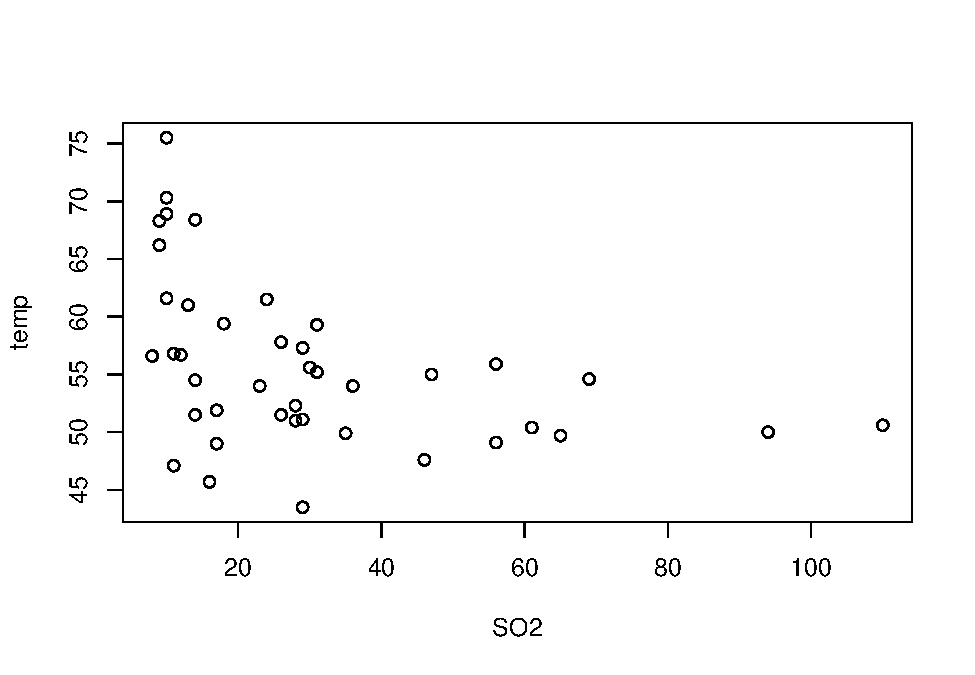
\includegraphics[width=0.33\linewidth,height=0.25\textheight]{HUDM6122-Homework_02-Chenguang-Pan_files/figure-latex/unnamed-chunk-3-1}
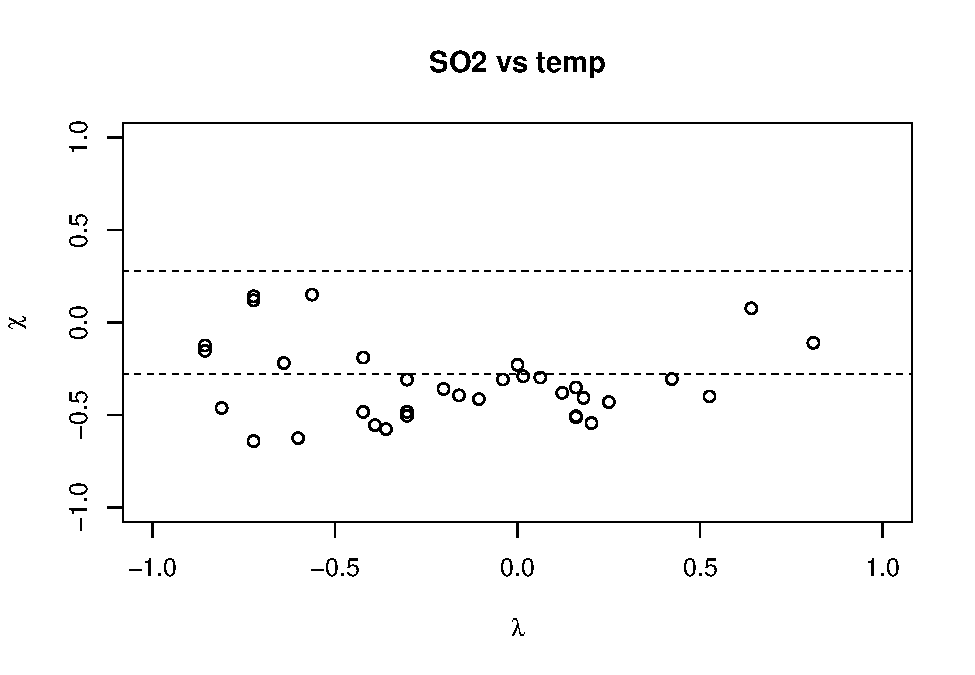
\includegraphics[width=0.33\linewidth,height=0.25\textheight]{HUDM6122-Homework_02-Chenguang-Pan_files/figure-latex/unnamed-chunk-3-2}
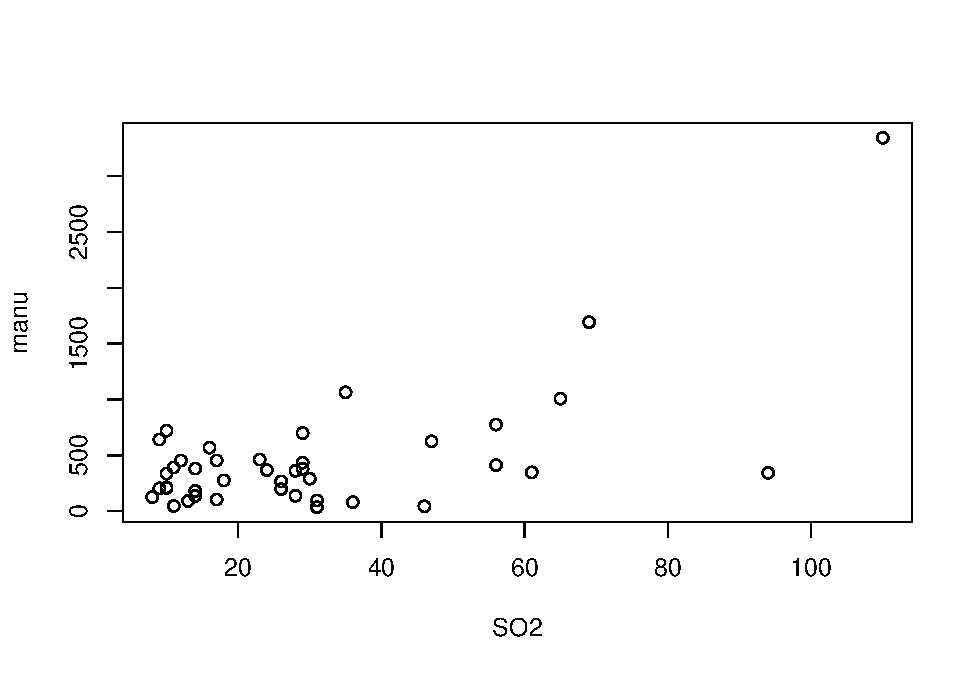
\includegraphics[width=0.33\linewidth,height=0.25\textheight]{HUDM6122-Homework_02-Chenguang-Pan_files/figure-latex/unnamed-chunk-3-3}
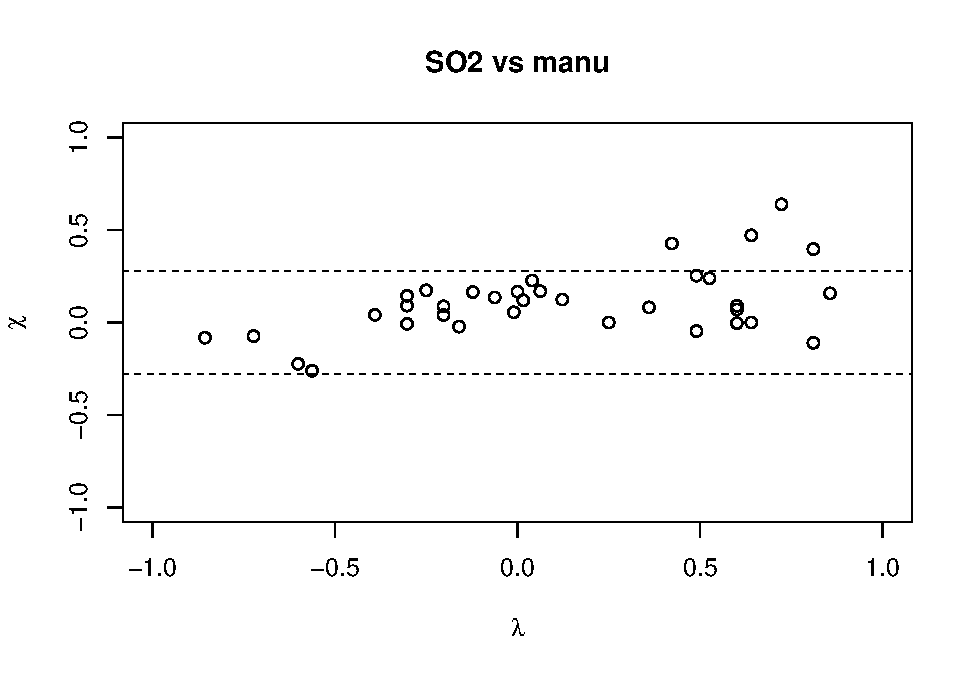
\includegraphics[width=0.33\linewidth,height=0.25\textheight]{HUDM6122-Homework_02-Chenguang-Pan_files/figure-latex/unnamed-chunk-3-4}
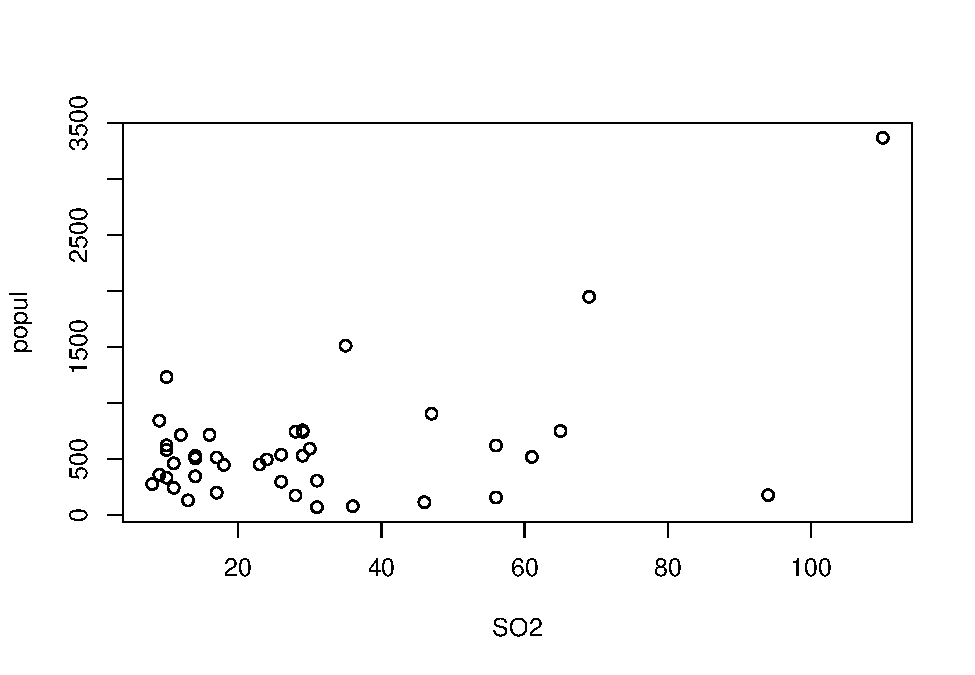
\includegraphics[width=0.33\linewidth,height=0.25\textheight]{HUDM6122-Homework_02-Chenguang-Pan_files/figure-latex/unnamed-chunk-3-5}
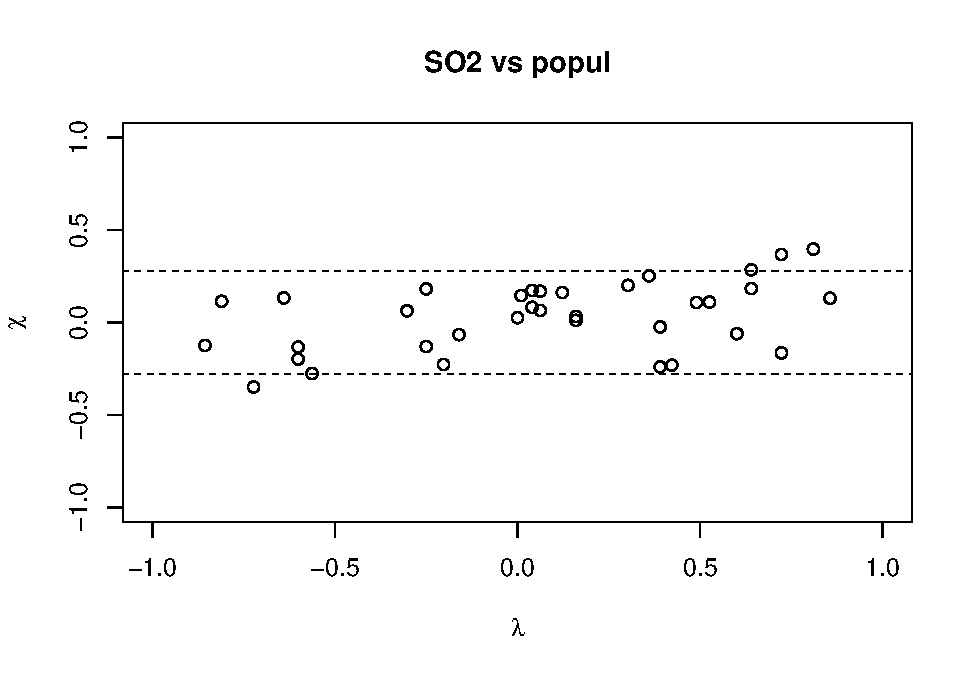
\includegraphics[width=0.33\linewidth,height=0.25\textheight]{HUDM6122-Homework_02-Chenguang-Pan_files/figure-latex/unnamed-chunk-3-6}
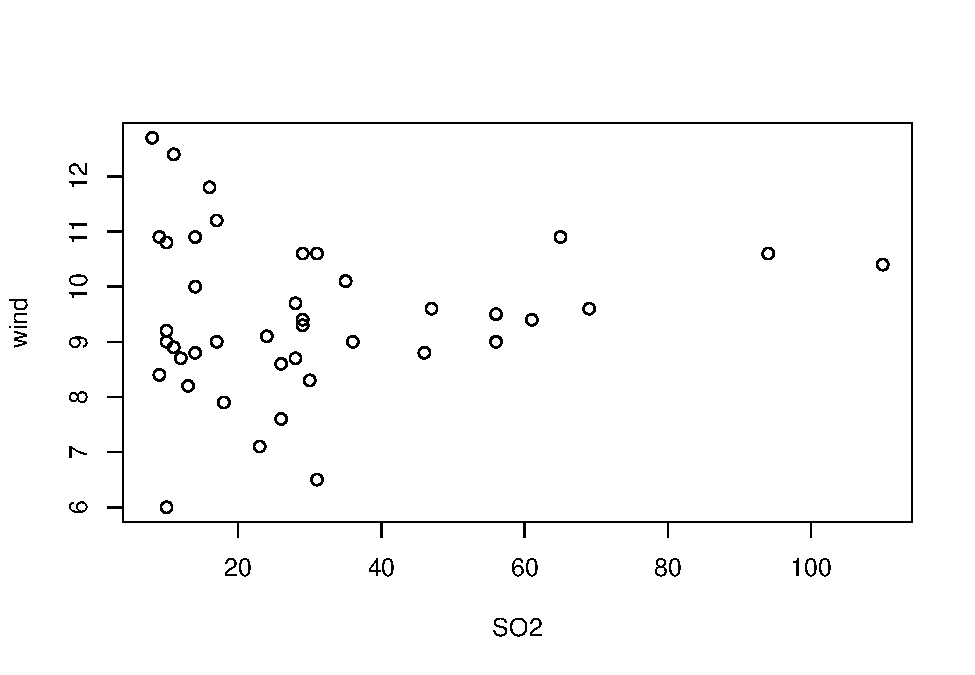
\includegraphics[width=0.33\linewidth,height=0.25\textheight]{HUDM6122-Homework_02-Chenguang-Pan_files/figure-latex/unnamed-chunk-3-7}
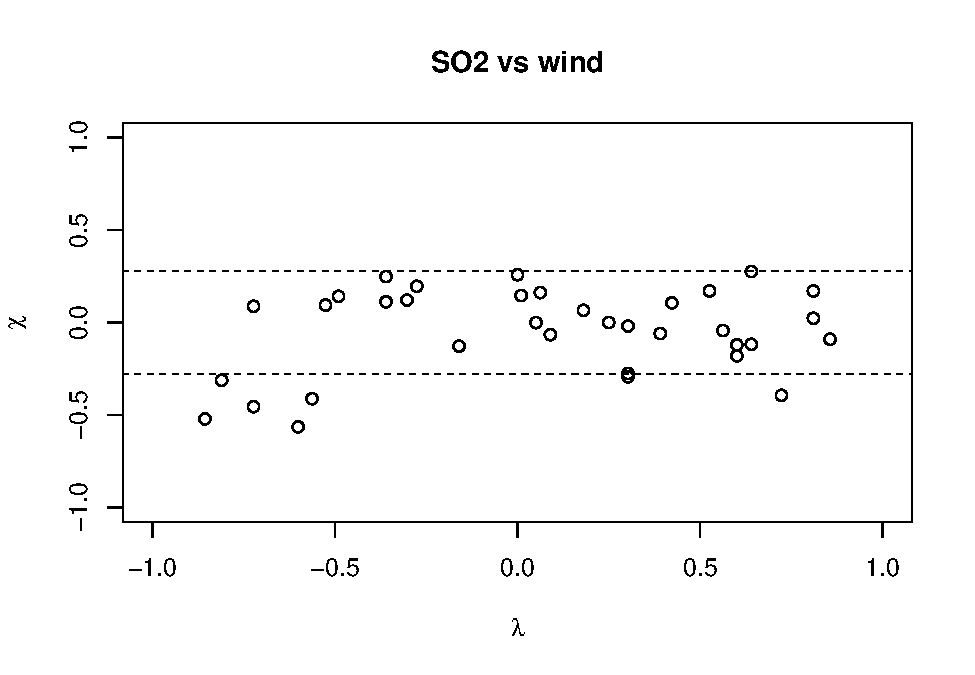
\includegraphics[width=0.33\linewidth,height=0.25\textheight]{HUDM6122-Homework_02-Chenguang-Pan_files/figure-latex/unnamed-chunk-3-8}
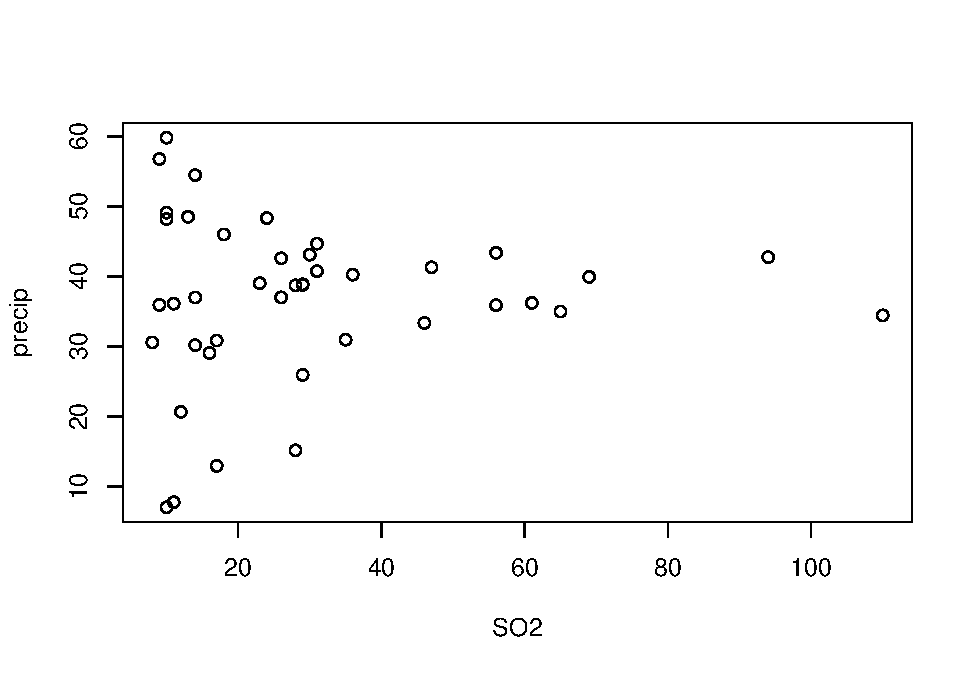
\includegraphics[width=0.33\linewidth,height=0.25\textheight]{HUDM6122-Homework_02-Chenguang-Pan_files/figure-latex/unnamed-chunk-3-9}
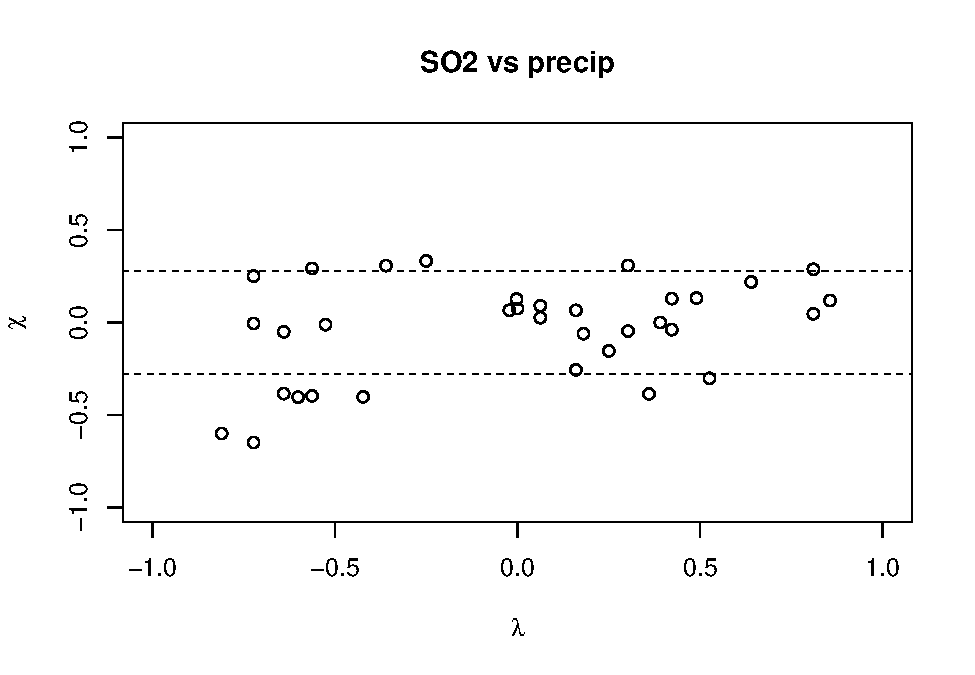
\includegraphics[width=0.33\linewidth,height=0.25\textheight]{HUDM6122-Homework_02-Chenguang-Pan_files/figure-latex/unnamed-chunk-3-10}
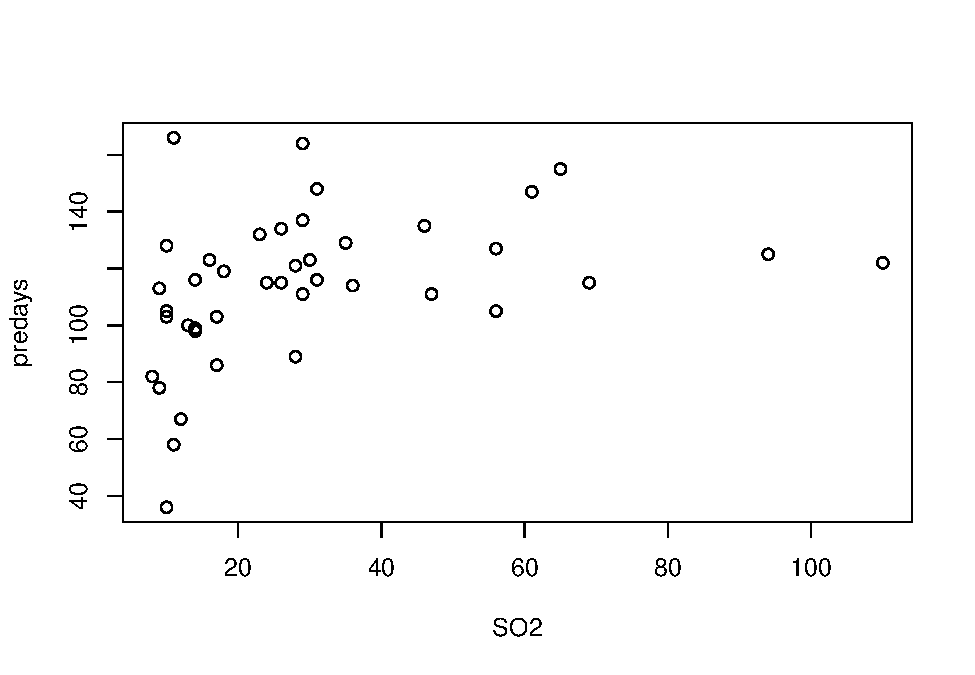
\includegraphics[width=0.33\linewidth,height=0.25\textheight]{HUDM6122-Homework_02-Chenguang-Pan_files/figure-latex/unnamed-chunk-3-11}
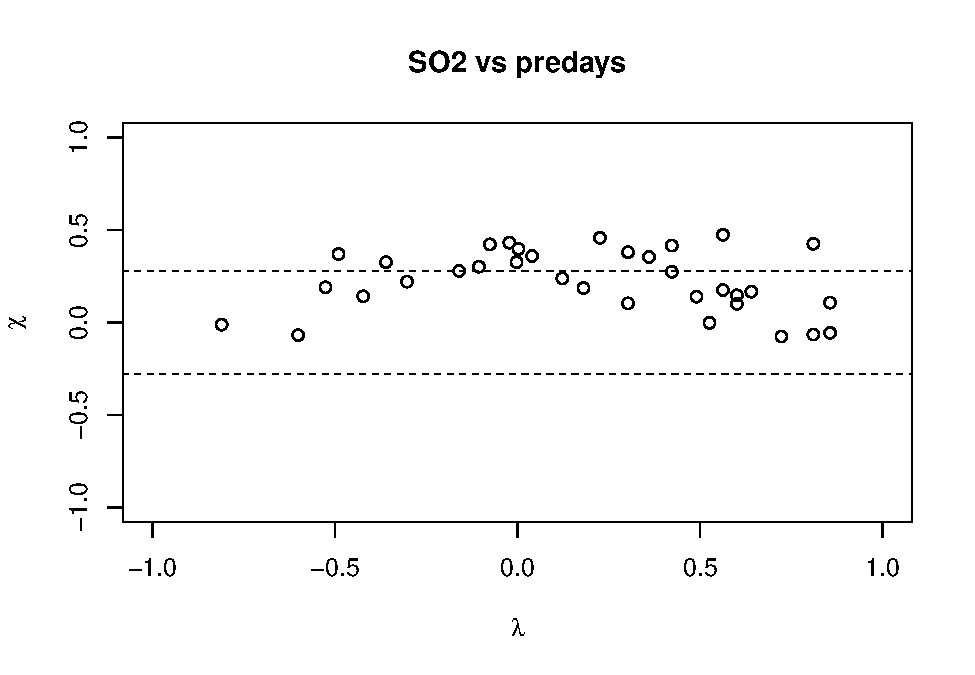
\includegraphics[width=0.33\linewidth,height=0.25\textheight]{HUDM6122-Homework_02-Chenguang-Pan_files/figure-latex/unnamed-chunk-3-12}
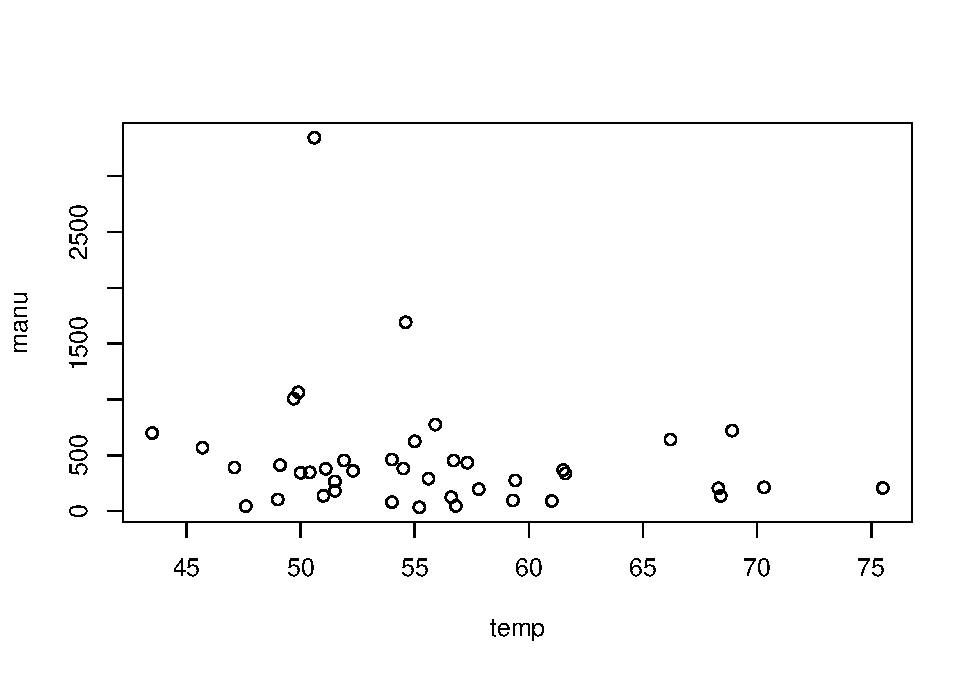
\includegraphics[width=0.33\linewidth,height=0.25\textheight]{HUDM6122-Homework_02-Chenguang-Pan_files/figure-latex/unnamed-chunk-3-13}
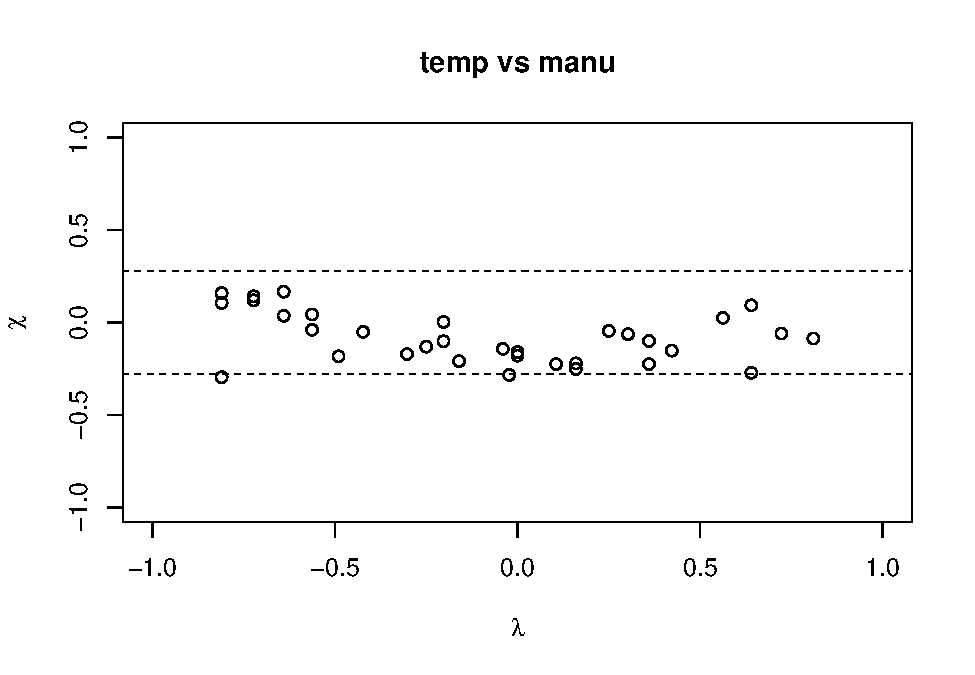
\includegraphics[width=0.33\linewidth,height=0.25\textheight]{HUDM6122-Homework_02-Chenguang-Pan_files/figure-latex/unnamed-chunk-3-14}
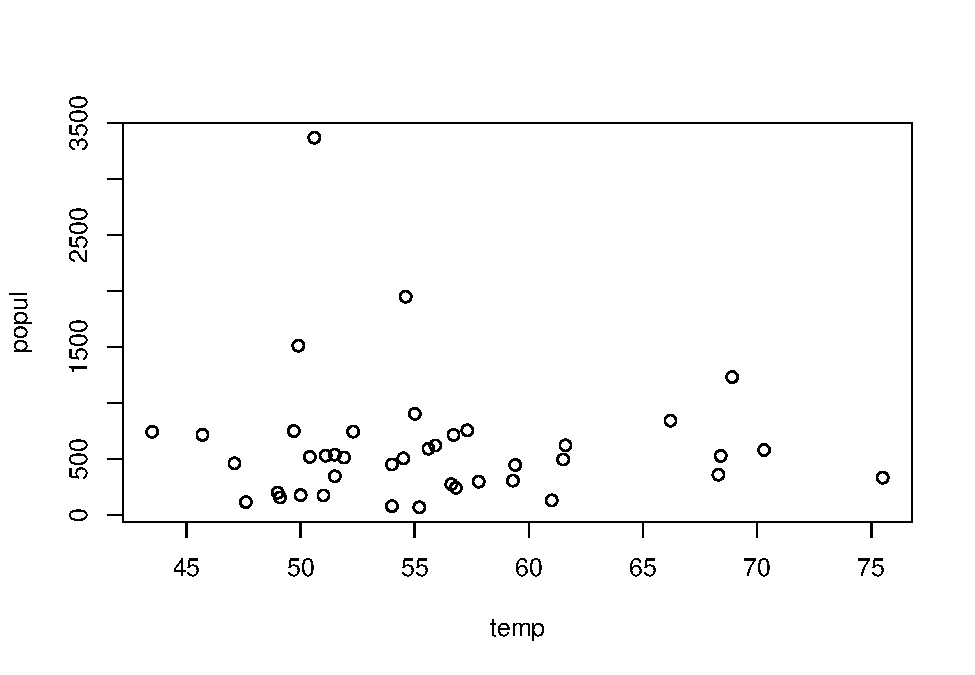
\includegraphics[width=0.33\linewidth,height=0.25\textheight]{HUDM6122-Homework_02-Chenguang-Pan_files/figure-latex/unnamed-chunk-3-15}
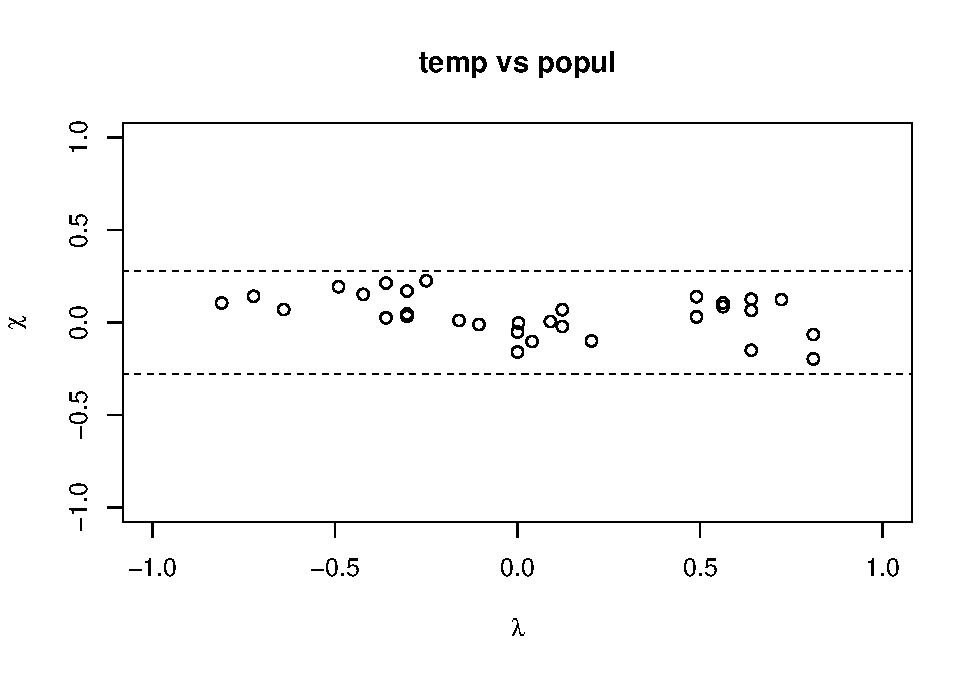
\includegraphics[width=0.33\linewidth,height=0.25\textheight]{HUDM6122-Homework_02-Chenguang-Pan_files/figure-latex/unnamed-chunk-3-16}
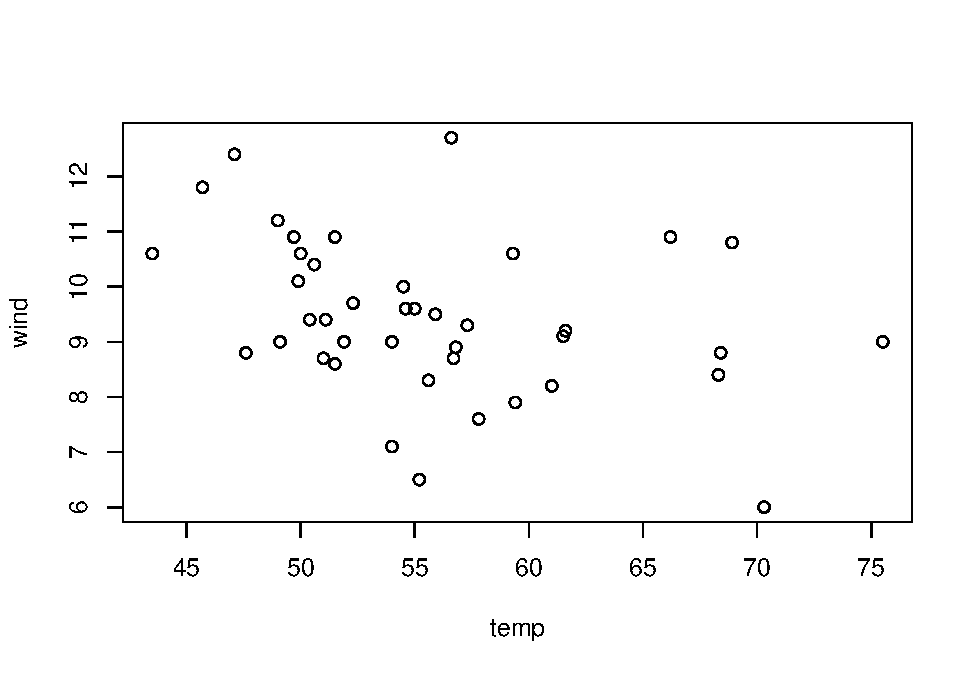
\includegraphics[width=0.33\linewidth,height=0.25\textheight]{HUDM6122-Homework_02-Chenguang-Pan_files/figure-latex/unnamed-chunk-3-17}
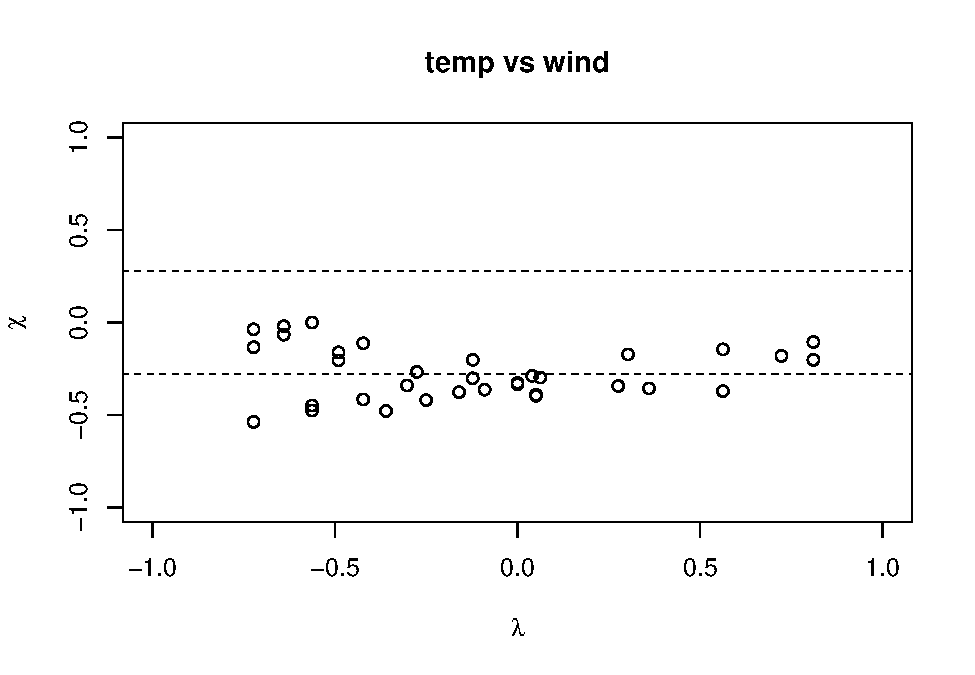
\includegraphics[width=0.33\linewidth,height=0.25\textheight]{HUDM6122-Homework_02-Chenguang-Pan_files/figure-latex/unnamed-chunk-3-18}
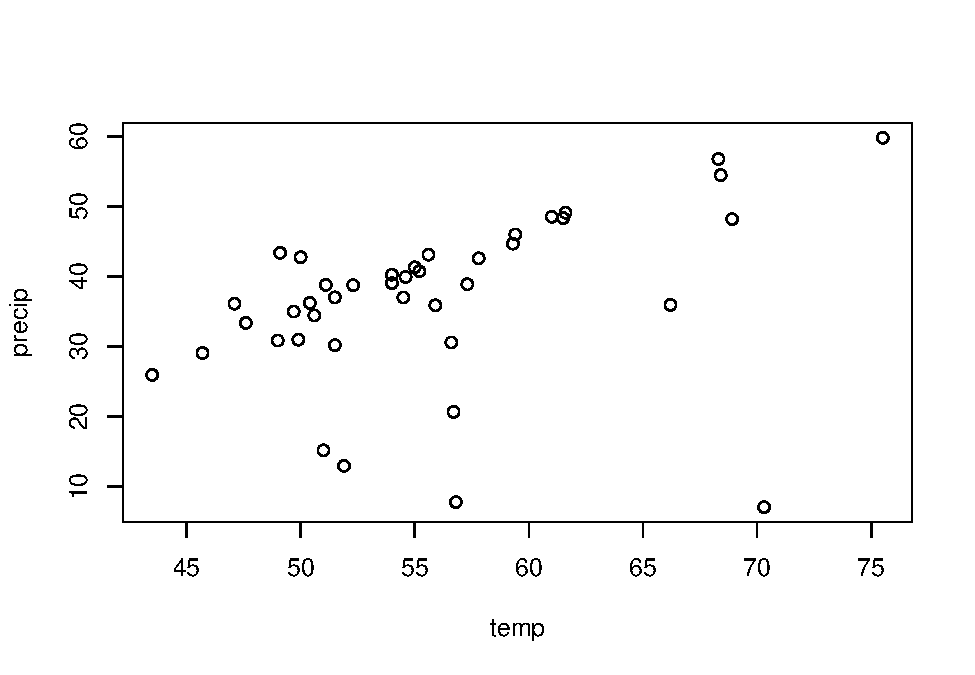
\includegraphics[width=0.33\linewidth,height=0.25\textheight]{HUDM6122-Homework_02-Chenguang-Pan_files/figure-latex/unnamed-chunk-3-19}
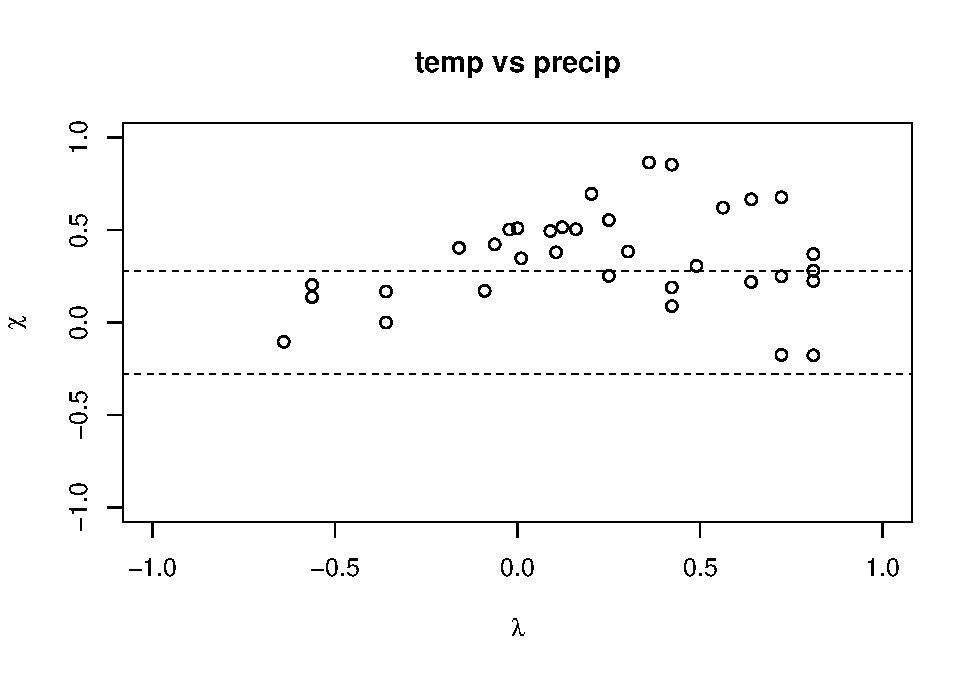
\includegraphics[width=0.33\linewidth,height=0.25\textheight]{HUDM6122-Homework_02-Chenguang-Pan_files/figure-latex/unnamed-chunk-3-20}
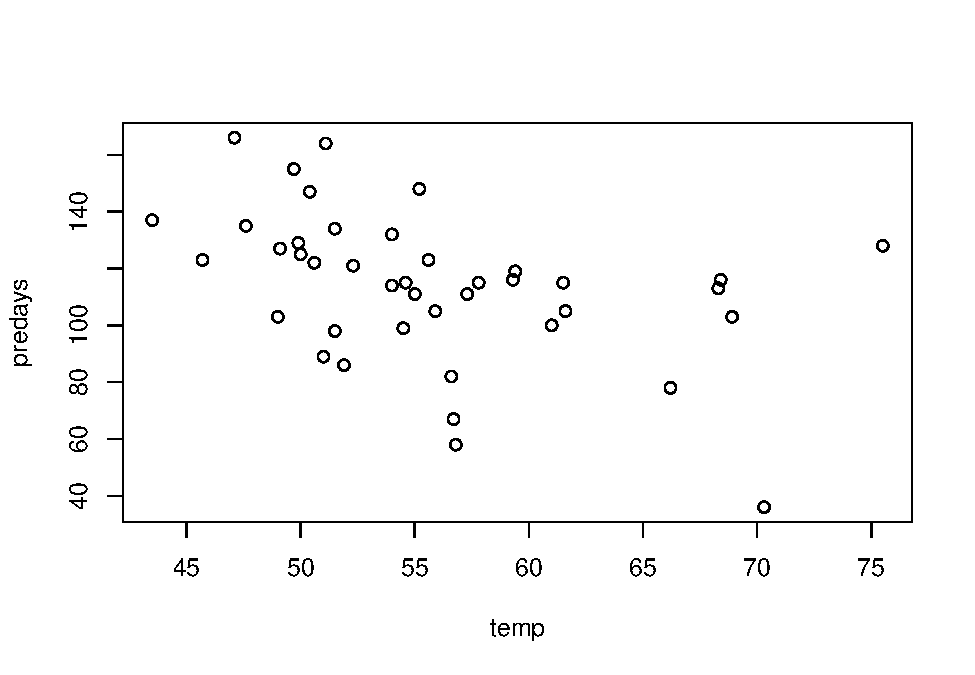
\includegraphics[width=0.33\linewidth,height=0.25\textheight]{HUDM6122-Homework_02-Chenguang-Pan_files/figure-latex/unnamed-chunk-3-21}
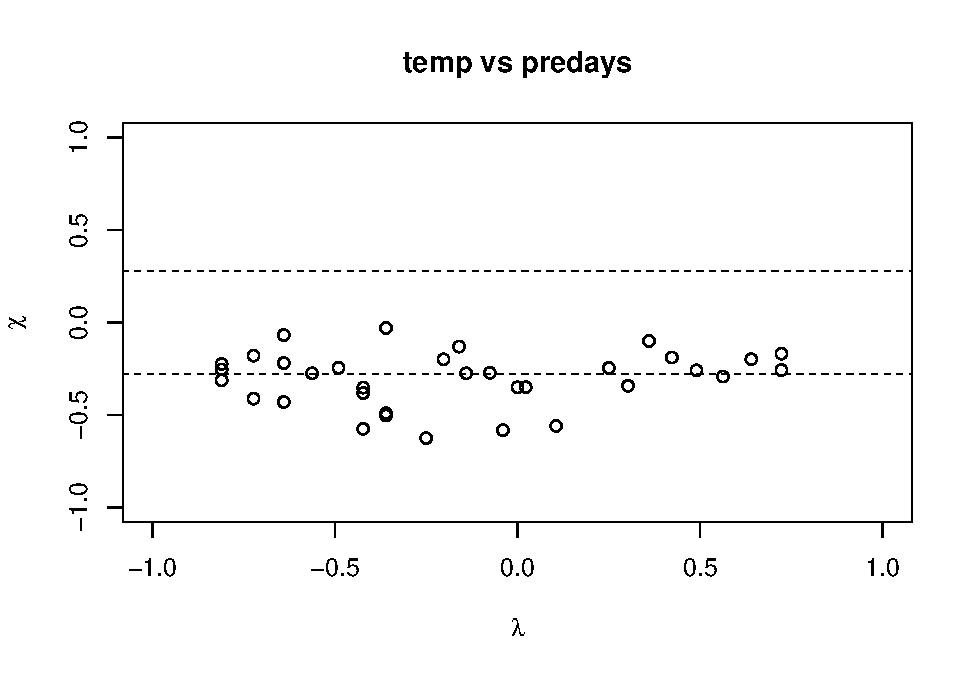
\includegraphics[width=0.33\linewidth,height=0.25\textheight]{HUDM6122-Homework_02-Chenguang-Pan_files/figure-latex/unnamed-chunk-3-22}
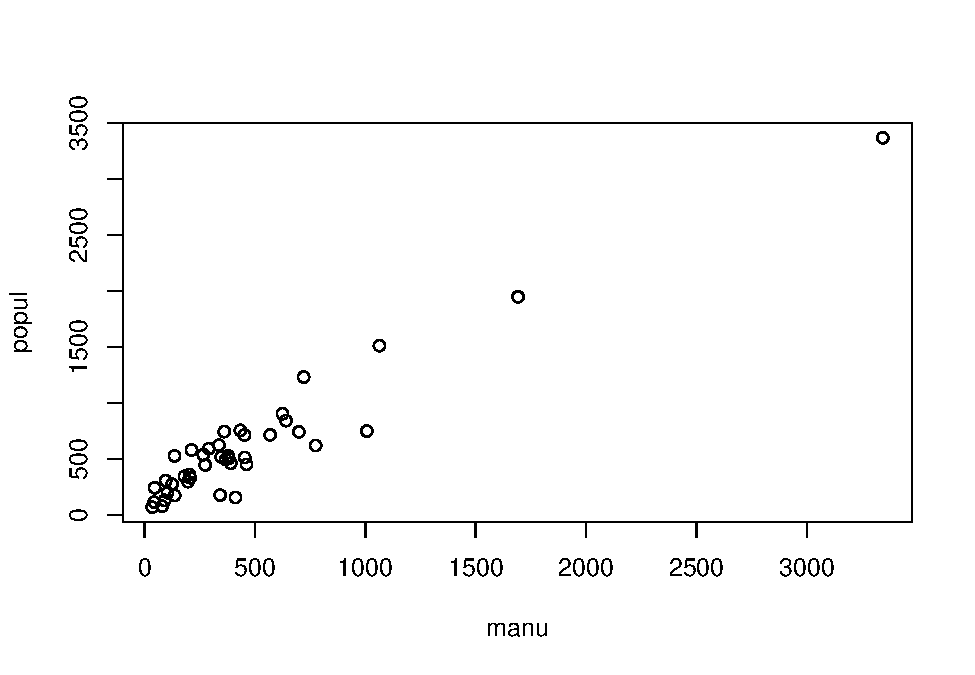
\includegraphics[width=0.33\linewidth,height=0.25\textheight]{HUDM6122-Homework_02-Chenguang-Pan_files/figure-latex/unnamed-chunk-3-23}
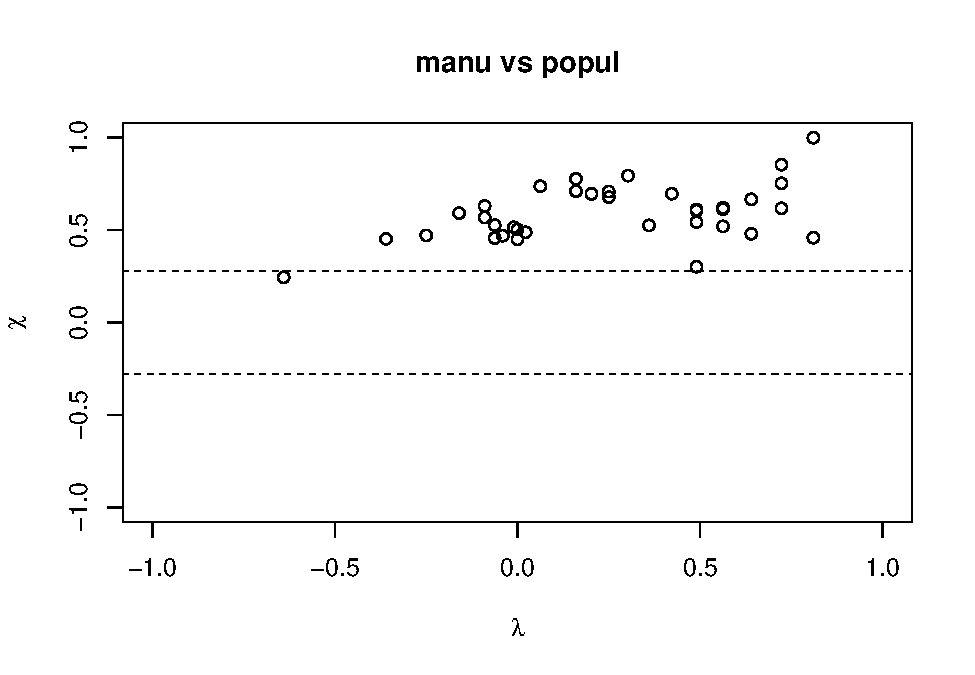
\includegraphics[width=0.33\linewidth,height=0.25\textheight]{HUDM6122-Homework_02-Chenguang-Pan_files/figure-latex/unnamed-chunk-3-24}
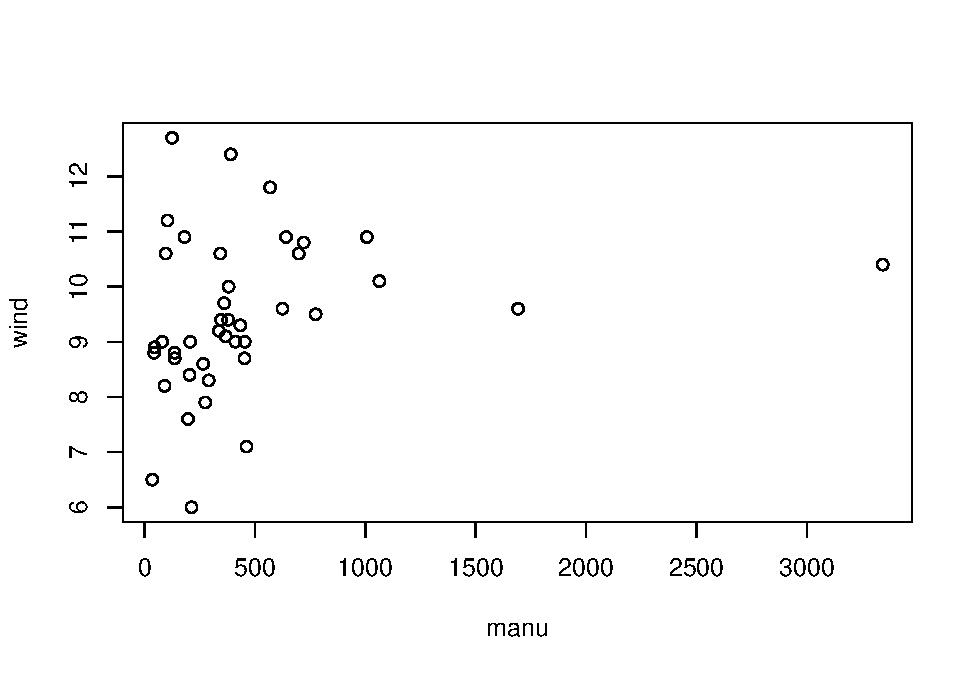
\includegraphics[width=0.33\linewidth,height=0.25\textheight]{HUDM6122-Homework_02-Chenguang-Pan_files/figure-latex/unnamed-chunk-3-25}
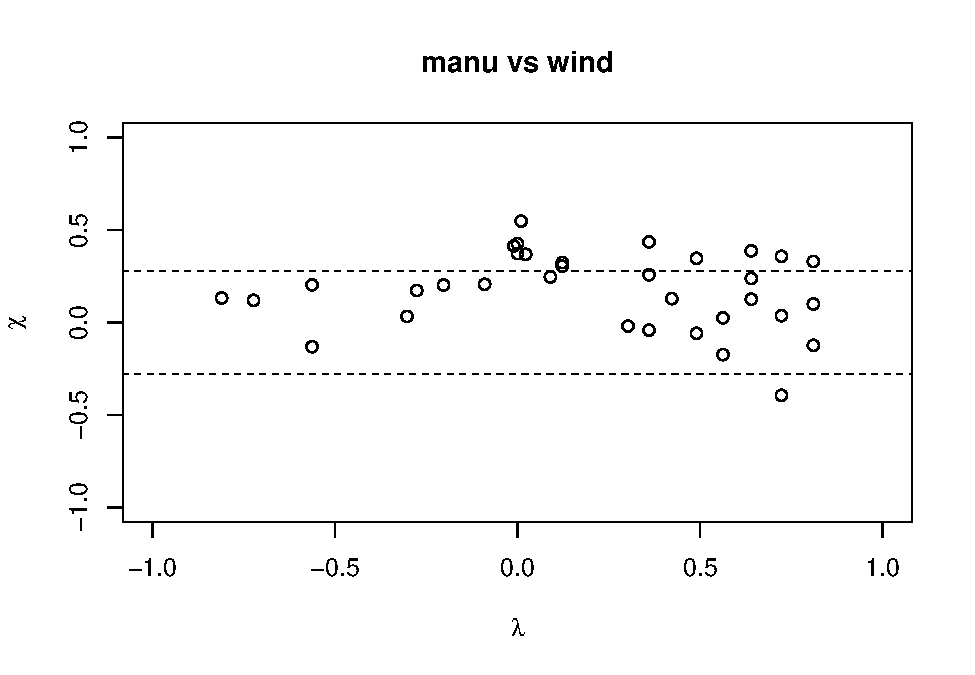
\includegraphics[width=0.33\linewidth,height=0.25\textheight]{HUDM6122-Homework_02-Chenguang-Pan_files/figure-latex/unnamed-chunk-3-26}
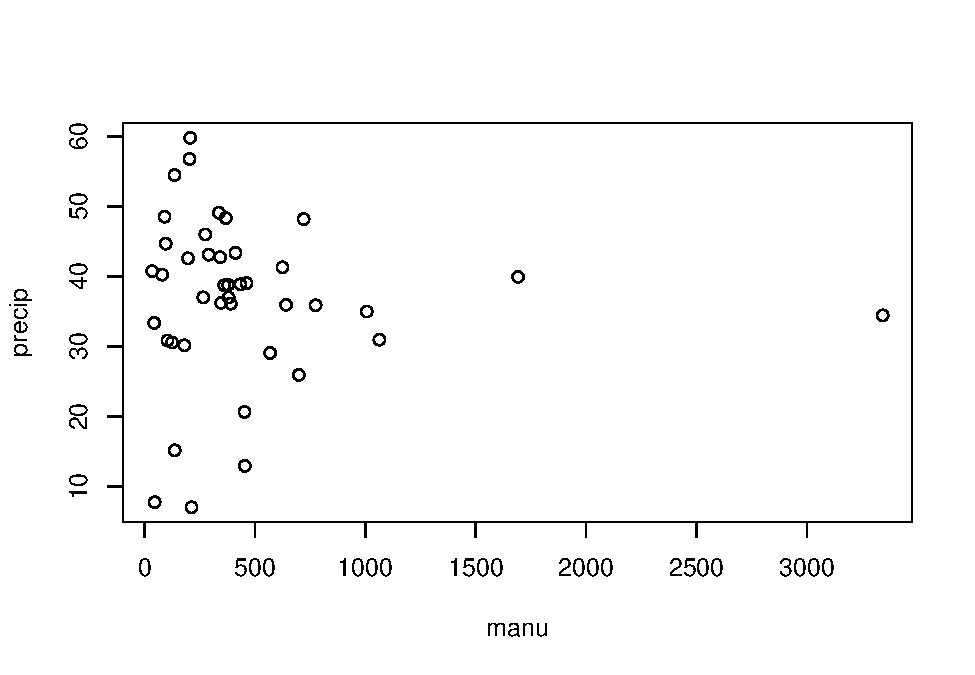
\includegraphics[width=0.33\linewidth,height=0.25\textheight]{HUDM6122-Homework_02-Chenguang-Pan_files/figure-latex/unnamed-chunk-3-27}
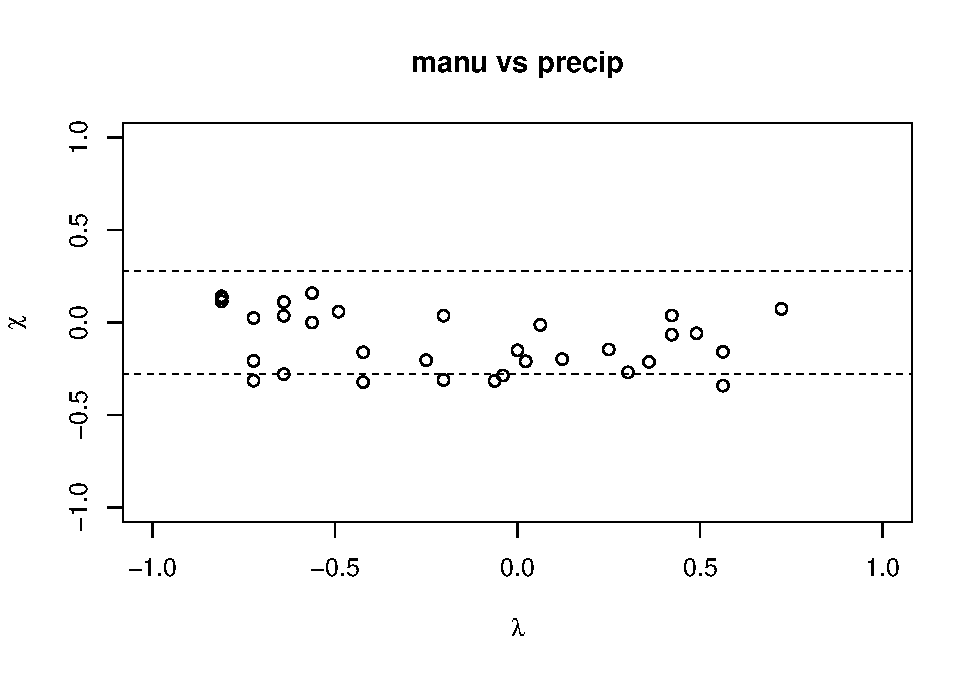
\includegraphics[width=0.33\linewidth,height=0.25\textheight]{HUDM6122-Homework_02-Chenguang-Pan_files/figure-latex/unnamed-chunk-3-28}
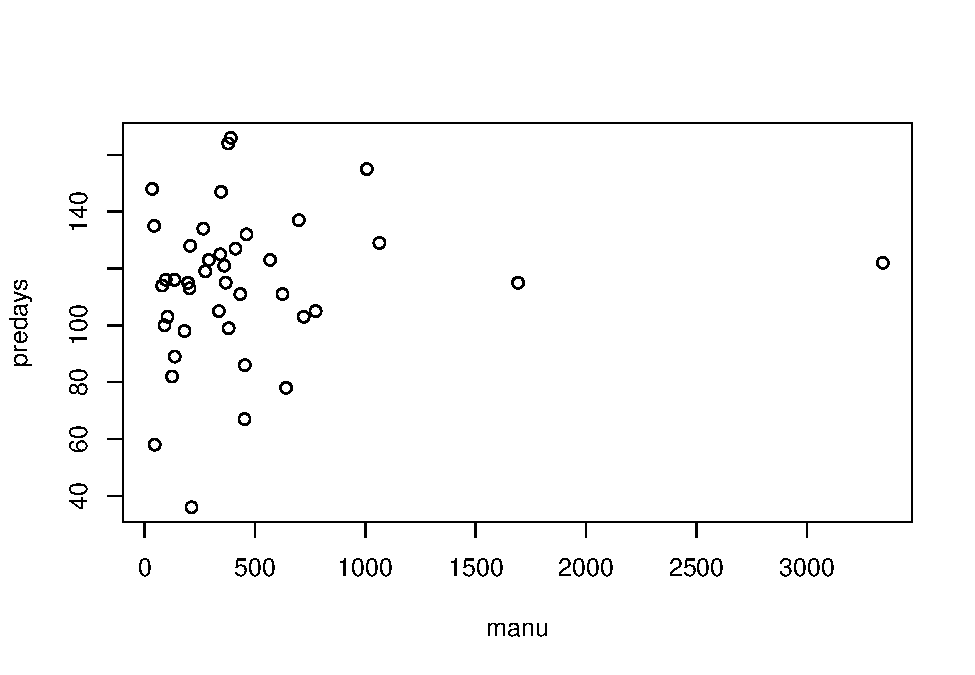
\includegraphics[width=0.33\linewidth,height=0.25\textheight]{HUDM6122-Homework_02-Chenguang-Pan_files/figure-latex/unnamed-chunk-3-29}
\includegraphics[width=0.33\linewidth,height=0.25\textheight]{HUDM6122-Homework_02-Chenguang-Pan_files/figure-latex/unnamed-chunk-3-30}
\includegraphics[width=0.33\linewidth,height=0.25\textheight]{HUDM6122-Homework_02-Chenguang-Pan_files/figure-latex/unnamed-chunk-3-31}
\includegraphics[width=0.33\linewidth,height=0.25\textheight]{HUDM6122-Homework_02-Chenguang-Pan_files/figure-latex/unnamed-chunk-3-32}
\includegraphics[width=0.33\linewidth,height=0.25\textheight]{HUDM6122-Homework_02-Chenguang-Pan_files/figure-latex/unnamed-chunk-3-33}
\includegraphics[width=0.33\linewidth,height=0.25\textheight]{HUDM6122-Homework_02-Chenguang-Pan_files/figure-latex/unnamed-chunk-3-34}
\includegraphics[width=0.33\linewidth,height=0.25\textheight]{HUDM6122-Homework_02-Chenguang-Pan_files/figure-latex/unnamed-chunk-3-35}
\includegraphics[width=0.33\linewidth,height=0.25\textheight]{HUDM6122-Homework_02-Chenguang-Pan_files/figure-latex/unnamed-chunk-3-36}
\includegraphics[width=0.33\linewidth,height=0.25\textheight]{HUDM6122-Homework_02-Chenguang-Pan_files/figure-latex/unnamed-chunk-3-37}
\includegraphics[width=0.33\linewidth,height=0.25\textheight]{HUDM6122-Homework_02-Chenguang-Pan_files/figure-latex/unnamed-chunk-3-38}
\includegraphics[width=0.33\linewidth,height=0.25\textheight]{HUDM6122-Homework_02-Chenguang-Pan_files/figure-latex/unnamed-chunk-3-39}
\includegraphics[width=0.33\linewidth,height=0.25\textheight]{HUDM6122-Homework_02-Chenguang-Pan_files/figure-latex/unnamed-chunk-3-40}
\includegraphics[width=0.33\linewidth,height=0.25\textheight]{HUDM6122-Homework_02-Chenguang-Pan_files/figure-latex/unnamed-chunk-3-41}
\includegraphics[width=0.33\linewidth,height=0.25\textheight]{HUDM6122-Homework_02-Chenguang-Pan_files/figure-latex/unnamed-chunk-3-42}
From the results, one can easily find that the scatter plots are
sometimes difficult to identify the independence between two variables.
But, comparatively the \texttt{chiplot} presents more straightforward
way to tell this attribute. For example, it is hard to find the relation
from the scattorplot for \texttt{manu} and \texttt{predays}, but the
chiplot clearly demonstrates that these two varriables are independent.

\hypertarget{ex.-2.3}{%
\subsection{Ex. 2.3}\label{ex.-2.3}}

\emph{Construct a scatterplot matrix of the body measurements data that
has the appropriate boxplot on the diagonal panels and bivariate
boxplots on the other panels. Compare the plot with Figure 2.17, and say
which diagram you find more informative about the data.}

\textbf{MY SOLUTION:}\\
The body measure dataset is not included in any packages. We need to
create the dataset by ourselves. First, based on the codes offered by
Prof.~Motta, Giovanni, I created measure data

\begin{Shaded}
\begin{Highlighting}[]
\SpecialCharTok{\textgreater{}} \CommentTok{\# create the  body measure data. Codes offered by Prof.Motta.}
\ErrorTok{\textgreater{}}\NormalTok{ measure }\OtherTok{\textless{}{-}}
\SpecialCharTok{+}   \FunctionTok{structure}\NormalTok{(}\FunctionTok{list}\NormalTok{(}\AttributeTok{V1 =} \DecValTok{1}\SpecialCharTok{:}\DecValTok{20}\NormalTok{, }\AttributeTok{V2 =} \FunctionTok{c}\NormalTok{(34L, 37L, 38L, 36L, 38L, 43L,}
\SpecialCharTok{+}\NormalTok{                  40L, 38L, 40L, 41L, 36L, 36L, 34L, 33L, 36L, 37L, 34L, 36L, 38L,}
\SpecialCharTok{+}\NormalTok{                  35L), }\AttributeTok{V3 =} \FunctionTok{c}\NormalTok{(30L, 32L, 30L, 33L, 29L, 32L, 33L, 30L, 30L, 32L,}
\SpecialCharTok{+}\NormalTok{                  24L, 25L, 24L, 22L, 26L, 26L, 25L, 26L, 28L, 23L), }\AttributeTok{V4 =} \FunctionTok{c}\NormalTok{(32L,}
\SpecialCharTok{+}\NormalTok{                  37L, 36L, 39L, 33L, 38L, 42L, 40L, 37L, 39L, 35L, 37L, 37L, 34L,}
\SpecialCharTok{+}\NormalTok{                  38L, 37L, 38L, 37L, 40L, 35L)), }\AttributeTok{.Names =} \FunctionTok{c}\NormalTok{(}\StringTok{"V1"}\NormalTok{, }\StringTok{"V2"}\NormalTok{, }\StringTok{"V3"}\NormalTok{,}
\SpecialCharTok{+}                  \StringTok{"V4"}\NormalTok{), }\AttributeTok{class =} \StringTok{"data.frame"}\NormalTok{, }\AttributeTok{row.names =} \FunctionTok{c}\NormalTok{(}\ConstantTok{NA}\NormalTok{, }\SpecialCharTok{{-}}\NormalTok{20L))}
\SpecialCharTok{\textgreater{}}\NormalTok{ measure }\OtherTok{\textless{}{-}}\NormalTok{ measure[,}\SpecialCharTok{{-}}\DecValTok{1}\NormalTok{]}
\SpecialCharTok{\textgreater{}} \FunctionTok{names}\NormalTok{(measure) }\OtherTok{\textless{}{-}} \FunctionTok{c}\NormalTok{(}\StringTok{"chest"}\NormalTok{, }\StringTok{"waist"}\NormalTok{, }\StringTok{"hips"}\NormalTok{)}
\SpecialCharTok{\textgreater{}}\NormalTok{ measure}\SpecialCharTok{$}\NormalTok{gender }\OtherTok{\textless{}{-}} \FunctionTok{gl}\NormalTok{(}\DecValTok{2}\NormalTok{, }\DecValTok{10}\NormalTok{)}
\SpecialCharTok{\textgreater{}} \FunctionTok{levels}\NormalTok{(measure}\SpecialCharTok{$}\NormalTok{gender) }\OtherTok{\textless{}{-}} \FunctionTok{c}\NormalTok{(}\StringTok{"male"}\NormalTok{, }\StringTok{"female"}\NormalTok{)}
\SpecialCharTok{\textgreater{}} 
\ErrorTok{\textgreater{}} \CommentTok{\# to only extract the continuous data}
\ErrorTok{\textgreater{}}\NormalTok{ measures }\OtherTok{\textless{}{-}}\NormalTok{ measure[,}\FunctionTok{c}\NormalTok{(}\DecValTok{1}\SpecialCharTok{:}\DecValTok{3}\NormalTok{)]}
\SpecialCharTok{\textgreater{}} \FunctionTok{par}\NormalTok{(}\AttributeTok{mfrow=}\FunctionTok{c}\NormalTok{(}\DecValTok{3}\NormalTok{, }\DecValTok{3}\NormalTok{))}
\SpecialCharTok{\textgreater{}} \ControlFlowTok{for}\NormalTok{ (i }\ControlFlowTok{in} \DecValTok{1}\SpecialCharTok{:}\DecValTok{3}\NormalTok{) \{}
\SpecialCharTok{+}   \ControlFlowTok{for}\NormalTok{ (j }\ControlFlowTok{in} \DecValTok{1}\SpecialCharTok{:}\FunctionTok{ncol}\NormalTok{(measures)) \{}
\SpecialCharTok{+}     \ControlFlowTok{if}\NormalTok{(i }\SpecialCharTok{!=}\NormalTok{ j) \{}
\SpecialCharTok{+}       \FunctionTok{bvbox}\NormalTok{(measures[, }\FunctionTok{c}\NormalTok{(i, j)])}
\SpecialCharTok{+}\NormalTok{     \}}
\SpecialCharTok{+}     \ControlFlowTok{else}\NormalTok{ \{}
\SpecialCharTok{+}       \FunctionTok{boxplot}\NormalTok{(measures[[i]])}
\SpecialCharTok{+}\NormalTok{     \}}
\SpecialCharTok{+}\NormalTok{   \}}
\SpecialCharTok{+}\NormalTok{ \}}
\end{Highlighting}
\end{Shaded}

\includegraphics{HUDM6122-Homework_02-Chenguang-Pan_files/figure-latex/unnamed-chunk-4-1.pdf}
It is quite challenging to draw the graph in the author's way! First,
\texttt{par("usr")} will return the coordiante of your current plot in
the unit your data in \texttt{(xmin,xmax,ymin,ymax)} order.

This scatterplot matrix can easily help reader find the outlier and the
descriptive information of each variable, like the quantile. In
contrasr, the figure 2.17 can help reader to find the joint distribution
of each pair and the distribution of the variable itself. I tend to
think the plot above is more infomrative.

\hypertarget{ex.-2.4}{%
\subsection{Ex. 2.4}\label{ex.-2.4}}

\emph{Construct a further scatterplot matrix of the body measurements
data that labels each point in a panel with the gender of the
individual, and plot on each scatterplot the separate estimated
bivariate densities for men and women.}

\textbf{MY SOLUTION:}

\begin{Shaded}
\begin{Highlighting}[]
\SpecialCharTok{\textgreater{}}\NormalTok{ ncols }\OtherTok{\textless{}{-}} \DecValTok{3} \CommentTok{\# only the first 3 columns are numeric}
\SpecialCharTok{\textgreater{}} \FunctionTok{par}\NormalTok{(}\AttributeTok{mfrow=}\FunctionTok{c}\NormalTok{(ncols, ncols))}
\SpecialCharTok{\textgreater{}} \ControlFlowTok{for}\NormalTok{ (i }\ControlFlowTok{in} \DecValTok{1}\SpecialCharTok{:}\NormalTok{ncols) \{}
\SpecialCharTok{+}   \ControlFlowTok{for}\NormalTok{ (j }\ControlFlowTok{in} \DecValTok{1}\SpecialCharTok{:}\NormalTok{ncols) \{}
\SpecialCharTok{+}     \FunctionTok{plot}\NormalTok{(measure[, i], measure[, j], }\AttributeTok{xlab =} \FunctionTok{names}\NormalTok{(measure)[i], }\AttributeTok{ylab=}\FunctionTok{names}\NormalTok{(measure)[j])}
\SpecialCharTok{+}     \ControlFlowTok{if}\NormalTok{(i }\SpecialCharTok{!=}\NormalTok{ j) \{}
\SpecialCharTok{+}       \FunctionTok{bvbox}\NormalTok{(measure[measure}\SpecialCharTok{$}\NormalTok{gender }\SpecialCharTok{==} \StringTok{"male"}\NormalTok{, }\FunctionTok{c}\NormalTok{(i, j)], }\AttributeTok{add=}\ConstantTok{TRUE}\NormalTok{)}
\SpecialCharTok{+}       \FunctionTok{bvbox}\NormalTok{(measure[measure}\SpecialCharTok{$}\NormalTok{gender }\SpecialCharTok{==} \StringTok{"female"}\NormalTok{, }\FunctionTok{c}\NormalTok{(i, j)], }\AttributeTok{add=}\ConstantTok{TRUE}\NormalTok{)}
\SpecialCharTok{+}\NormalTok{     \}}
\SpecialCharTok{+}     \FunctionTok{points}\NormalTok{(measure[measure}\SpecialCharTok{$}\NormalTok{gender }\SpecialCharTok{==} \StringTok{"male"}\NormalTok{, }\FunctionTok{c}\NormalTok{(i, j)], }\AttributeTok{col=}\StringTok{"blue"}\NormalTok{)}
\SpecialCharTok{+}     \FunctionTok{points}\NormalTok{(measure[measure}\SpecialCharTok{$}\NormalTok{gender }\SpecialCharTok{==} \StringTok{"female"}\NormalTok{, }\FunctionTok{c}\NormalTok{(i, j)], }\AttributeTok{col=}\StringTok{"red"}\NormalTok{)}
\SpecialCharTok{+}\NormalTok{   \}}
\SpecialCharTok{+}\NormalTok{ \}}
\end{Highlighting}
\end{Shaded}

\includegraphics{HUDM6122-Homework_02-Chenguang-Pan_files/figure-latex/unnamed-chunk-6-1.pdf}

\hypertarget{ex.-2.5}{%
\subsection{Ex. 2.5}\label{ex.-2.5}}

\emph{Construct a scatterplot matrix of the chemical composition of
Romano-British pottery given in Chapter 1 (Table 1.3), identifying each
unit by its kiln number and showing the estimated bivariate density on
each panel. What does the resulting diagram tell you?}

\textbf{MY SOLUTION:}

\begin{Shaded}
\begin{Highlighting}[]
\SpecialCharTok{\textgreater{}} \CommentTok{\# pairs(measure, panel = function(x, y) plot(density(cbind(x, y)), add = TRUE))}
\ErrorTok{\textgreater{}} \FunctionTok{library}\NormalTok{(}\StringTok{"KernSmooth"}\NormalTok{)}
\SpecialCharTok{\textgreater{}} \FunctionTok{par}\NormalTok{(}\AttributeTok{mar =} \FunctionTok{c}\NormalTok{(}\DecValTok{1}\NormalTok{, }\DecValTok{1}\NormalTok{, }\DecValTok{1}\NormalTok{, }\DecValTok{1}\NormalTok{))}
\SpecialCharTok{\textgreater{}}\NormalTok{ n }\OtherTok{=} \FunctionTok{ncol}\NormalTok{(pottery) }\SpecialCharTok{{-}} \DecValTok{1}
\SpecialCharTok{\textgreater{}} \FunctionTok{par}\NormalTok{(}\AttributeTok{mfrow =} \FunctionTok{c}\NormalTok{(n, n))}
\SpecialCharTok{\textgreater{}} \ControlFlowTok{for}\NormalTok{ (i }\ControlFlowTok{in} \DecValTok{1}\SpecialCharTok{:}\NormalTok{n) \{}
\SpecialCharTok{+}   \ControlFlowTok{for}\NormalTok{(j }\ControlFlowTok{in} \DecValTok{1}\SpecialCharTok{:}\NormalTok{n)\{}
\SpecialCharTok{+}     
\SpecialCharTok{+}     \ControlFlowTok{if}\NormalTok{(i }\SpecialCharTok{==}\NormalTok{ j)\{}
\SpecialCharTok{+}       \CommentTok{\#d = density(pottery[, i])}
\SpecialCharTok{+}       \CommentTok{\#plot(d, main = colnames(pottery)[i])}
\SpecialCharTok{+}       \CommentTok{\#text(d, cex = 0.6,}
\SpecialCharTok{+}            \CommentTok{\#labels = abbreviate(pottery$kiln))}
\SpecialCharTok{+}       \FunctionTok{par}\NormalTok{(}\AttributeTok{mar =} \FunctionTok{c}\NormalTok{(}\DecValTok{0}\NormalTok{,}\DecValTok{0}\NormalTok{,}\DecValTok{0}\NormalTok{,}\DecValTok{0}\NormalTok{))}
\SpecialCharTok{+}       \FunctionTok{plot}\NormalTok{(}\FunctionTok{c}\NormalTok{(}\DecValTok{0}\NormalTok{, }\DecValTok{1}\NormalTok{), }\FunctionTok{c}\NormalTok{(}\DecValTok{0}\NormalTok{, }\DecValTok{1}\NormalTok{), }\AttributeTok{ann =}\NormalTok{ F, }\AttributeTok{bty =} \StringTok{\textquotesingle{}n\textquotesingle{}}\NormalTok{, }\AttributeTok{type =} \StringTok{\textquotesingle{}n\textquotesingle{}}\NormalTok{, }\AttributeTok{xaxt =} \StringTok{\textquotesingle{}n\textquotesingle{}}\NormalTok{, }\AttributeTok{yaxt =} \StringTok{\textquotesingle{}n\textquotesingle{}}\NormalTok{)}
\SpecialCharTok{+}       
\SpecialCharTok{+}       \FunctionTok{text}\NormalTok{(}\AttributeTok{x =} \FloatTok{0.3}\NormalTok{, }\AttributeTok{y =} \FloatTok{0.5}\NormalTok{, }\FunctionTok{paste}\NormalTok{(}\FunctionTok{colnames}\NormalTok{(pottery)[i]), }
\SpecialCharTok{+}            \AttributeTok{cex =} \FloatTok{1.5}\NormalTok{, }\AttributeTok{col =} \StringTok{"black"}\NormalTok{, }\AttributeTok{family=}\StringTok{"serif"}\NormalTok{, }\AttributeTok{font=}\DecValTok{2}\NormalTok{, }\AttributeTok{adj=}\FloatTok{0.5}\NormalTok{)}
\SpecialCharTok{+}\NormalTok{     \}}
\SpecialCharTok{+}     \ControlFlowTok{else}\NormalTok{\{}
\SpecialCharTok{+}\NormalTok{       measured }\OtherTok{=} \FunctionTok{bkde2D}\NormalTok{(pottery[, }\FunctionTok{c}\NormalTok{(i, j)], }
\SpecialCharTok{+}                 \AttributeTok{bandwidth =} \FunctionTok{sapply}\NormalTok{(pottery[, }\FunctionTok{c}\NormalTok{(i, j)], dpik))}
\SpecialCharTok{+}       
\SpecialCharTok{+}       \FunctionTok{plot}\NormalTok{(pottery[, }\FunctionTok{c}\NormalTok{(i, j)],}
\SpecialCharTok{+}            \AttributeTok{xlab =} \FunctionTok{colnames}\NormalTok{(pottery)[i],}
\SpecialCharTok{+}            \AttributeTok{ylab =} \FunctionTok{colnames}\NormalTok{(pottery)[j])}
\SpecialCharTok{+}       \FunctionTok{contour}\NormalTok{(}\AttributeTok{x =}\NormalTok{ measured}\SpecialCharTok{$}\NormalTok{x1, }\AttributeTok{y =}\NormalTok{ measured}\SpecialCharTok{$}\NormalTok{x2,}
\SpecialCharTok{+}               \AttributeTok{z =}\NormalTok{ measured}\SpecialCharTok{$}\NormalTok{fhat, }\AttributeTok{add =} \ConstantTok{TRUE}\NormalTok{)}
\SpecialCharTok{+}       \FunctionTok{text}\NormalTok{(pottery[,i], pottery[,j], }\AttributeTok{cex =} \FloatTok{0.6}\NormalTok{,}
\SpecialCharTok{+}            \AttributeTok{labels =} \FunctionTok{abbreviate}\NormalTok{(pottery}\SpecialCharTok{$}\NormalTok{kiln))}
\SpecialCharTok{+}       
\SpecialCharTok{+}\NormalTok{     \}}
\SpecialCharTok{+}\NormalTok{   \}}
\SpecialCharTok{+}   
\SpecialCharTok{+}\NormalTok{ \}}
\end{Highlighting}
\end{Shaded}

\includegraphics{HUDM6122-Homework_02-Chenguang-Pan_files/figure-latex/unnamed-chunk-8-1.pdf}
The results is actually not very good-looking, but it still presents the
joint distribution of each pair. These joint distributions seems not
follow any regular probability distribution.

\hypertarget{ex.-2.6}{%
\subsection{Ex. 2.6}\label{ex.-2.6}}

\emph{Ex. 2.6 Construct a bubble plot of the earthquake data using
latitude and longitude as the scatterplot and depth as the circles, with
greater depths giving smaller circles. In addition, divide the
magnitudes into three equal ranges and label the points in your bubble
plot with a different symbol depending on the magnitude group into which
the point falls.}

\begin{Shaded}
\begin{Highlighting}[]
\SpecialCharTok{\textgreater{}} \FunctionTok{library}\NormalTok{(lattice)}
\SpecialCharTok{\textgreater{}} \FunctionTok{par}\NormalTok{(}\AttributeTok{mfrow =} \FunctionTok{c}\NormalTok{(}\DecValTok{1}\NormalTok{, }\DecValTok{1}\NormalTok{))}
\SpecialCharTok{\textgreater{}} \CommentTok{\#ylim \textless{}{-} with(quakes, range(long)) * c(0.95, 1)}
\ErrorTok{\textgreater{}}\NormalTok{ sub1 }\OtherTok{=} \FunctionTok{subset}\NormalTok{(quakes, }\AttributeTok{subset =}\NormalTok{ mag }\SpecialCharTok{\textgreater{}} \DecValTok{4} \SpecialCharTok{\&}\NormalTok{ mag }\SpecialCharTok{\textless{}=} \FloatTok{4.8}\NormalTok{)}
\SpecialCharTok{\textgreater{}}\NormalTok{ sub2 }\OtherTok{=} \FunctionTok{subset}\NormalTok{(quakes, }\AttributeTok{subset =}\NormalTok{ mag }\SpecialCharTok{\textgreater{}} \FloatTok{4.8} \SpecialCharTok{\&}\NormalTok{ mag }\SpecialCharTok{\textless{}=} \FloatTok{5.6}\NormalTok{)}
\SpecialCharTok{\textgreater{}}\NormalTok{ sub3 }\OtherTok{=} \FunctionTok{subset}\NormalTok{(quakes, }\AttributeTok{subset =}\NormalTok{ mag }\SpecialCharTok{\textgreater{}}\FloatTok{5.6} \SpecialCharTok{\&}\NormalTok{ mag }\SpecialCharTok{\textless{}=} \FloatTok{6.4}\NormalTok{)}
\SpecialCharTok{\textgreater{}} 
\ErrorTok{\textgreater{}} 
\ErrorTok{\textgreater{}} \FunctionTok{attach}\NormalTok{(quakes)}
\SpecialCharTok{\textgreater{}} \FunctionTok{plot}\NormalTok{(lat, long,}
\SpecialCharTok{+}      \AttributeTok{xlab =} \StringTok{"Latitude"}\NormalTok{,}\AttributeTok{ylab =} \StringTok{"Longitude"}\NormalTok{, }\AttributeTok{pch=}\DecValTok{10}\NormalTok{)}
\SpecialCharTok{\textgreater{}} 
\ErrorTok{\textgreater{}} \FunctionTok{with}\NormalTok{(sub1, }\FunctionTok{symbols}\NormalTok{(lat, long, }\AttributeTok{circles =} \DecValTok{1000}\SpecialCharTok{{-}}\NormalTok{ depth,}
\SpecialCharTok{+}                    \AttributeTok{inches =} \FloatTok{0.2}\NormalTok{, }\AttributeTok{add =}\NormalTok{ T, }\AttributeTok{fg=}\StringTok{"green"}\NormalTok{))}
\SpecialCharTok{\textgreater{}} \FunctionTok{with}\NormalTok{(sub2, }\FunctionTok{symbols}\NormalTok{(lat, long, }\AttributeTok{circles =} \DecValTok{1000}\SpecialCharTok{{-}}\NormalTok{ depth,}
\SpecialCharTok{+}                    \AttributeTok{inches =} \FloatTok{0.2}\NormalTok{, }\AttributeTok{add =}\NormalTok{ T, }\AttributeTok{fg=}\StringTok{"red"}\NormalTok{))}
\SpecialCharTok{\textgreater{}} \FunctionTok{with}\NormalTok{(sub3, }\FunctionTok{symbols}\NormalTok{(lat, long, }\AttributeTok{circles =} \DecValTok{1000}\SpecialCharTok{{-}}\NormalTok{ depth,}
\SpecialCharTok{+}                    \AttributeTok{inches =} \FloatTok{0.2}\NormalTok{, }\AttributeTok{add =}\NormalTok{ T, }\AttributeTok{fg=}\StringTok{"blue"}\NormalTok{))}
\SpecialCharTok{\textgreater{}} \FunctionTok{legend}\NormalTok{(}\SpecialCharTok{{-}}\DecValTok{38}\NormalTok{,}\DecValTok{173}\NormalTok{, }\AttributeTok{legend =} \FunctionTok{c}\NormalTok{(}\StringTok{"4 \textless{} mag \textless{}= 4.8"}\NormalTok{, }
\SpecialCharTok{+}                        \StringTok{"4.8 \textless{} mag \textless{}= 5.6"}\NormalTok{,}
\SpecialCharTok{+}                        \StringTok{"5.6 \textless{} mag \textless{}= 6.4"}\NormalTok{), }\AttributeTok{fill=}\FunctionTok{c}\NormalTok{(}\StringTok{"green"}\NormalTok{,}\StringTok{"red"}\NormalTok{,}\StringTok{"blue"}\NormalTok{))}
\end{Highlighting}
\end{Shaded}

\includegraphics{HUDM6122-Homework_02-Chenguang-Pan_files/figure-latex/unnamed-chunk-10-1.pdf}

\end{document}
